% ============================================================
%  DDH 超声图像智能裁剪系统 · 技术开发说明文档（第 2 版 / 论文式结构）
%  编译：xelatex → bibtex → xelatex ×2
%  结构：项目背景 → 设计目标 → 技术方案 → 研究方法 → 实验结果与讨论 → 创新性说明
% ============================================================
\documentclass[UTF8,a4paper,10pt]{ctexart}

\usepackage[left=2.05cm,right=2.05cm,top=2.10cm,bottom=1.95cm,headsep=0.45cm,footskip=0.85cm]{geometry}
\usepackage{amsmath,amssymb}
\usepackage{graphicx}
\usepackage{booktabs}
\usepackage{multirow}
\usepackage{array}
\usepackage{caption}
\usepackage{subcaption}
\usepackage{enumitem}
\usepackage{fancyhdr}
\usepackage{titlesec}
\usepackage{xcolor}
\usepackage{colortbl}
\usepackage{tikz}
\usetikzlibrary{calc,decorations.pathmorphing}
\usepackage[numbers,sort&compress]{gbt7714}
\usepackage[colorlinks=true,linkcolor=navy,citecolor=navy,urlcolor=navy]{hyperref}

\definecolor{navy}{HTML}{1F3864}
\definecolor{rust}{HTML}{A33A14}
\definecolor{teal}{HTML}{1F5C4D}
\definecolor{deco}{HTML}{E4EDF6}
\definecolor{decob}{HTML}{CBDCEE}

% ---------- 页面装饰 ----------
\AddToHook{shipout/background}{\put(0,0){%
\begin{tikzpicture}[remember picture,overlay]
  \draw[deco, line width=1.6pt, smooth]
    ($(current page.north west)+(0,-0.42cm)$) .. controls +(3.8cm,-0.24cm) and +(-3.8cm,0.22cm) ..
    ($(current page.north)+(0,-0.46cm)$)
    .. controls +(3.8cm,-0.22cm) and +(-3.8cm,0.24cm) .. ($(current page.north east)+(0,-0.42cm)$);
  \draw[deco, line width=1.6pt, smooth]
    ($(current page.south west)+(0,0.42cm)$) .. controls +(3.8cm,0.24cm) and +(-3.8cm,-0.22cm) ..
    ($(current page.south)+(0,0.46cm)$)
    .. controls +(3.8cm,0.22cm) and +(-3.8cm,-0.24cm) .. ($(current page.south east)+(0,0.42cm)$);
\end{tikzpicture}}}

\ctexset{
  section={format=\large\bfseries\sffamily\color{navy}, beforeskip=7pt plus 2pt, afterskip=4pt},
  subsection={format=\normalsize\bfseries\sffamily\color{navy!85!black}, beforeskip=5pt plus 1pt, afterskip=2.5pt},
}
\renewcommand{\thesection}{\arabic{section}}
\setlength{\parskip}{1.0pt}
\linespread{1.07}

\captionsetup{font=small,labelsep=quad,skip=3.5pt}
% ---- 图注/表注：浅灰蓝底纹 + 左侧细竖线（医学期刊常见处理） ----
\usepackage[framemethod=tikz]{mdframed}
\captionsetup[figure]{font=small,labelsep=quad,skip=3pt,singlelinecheck=false}
\captionsetup[table]{font=small,labelsep=quad,skip=2pt,aboveskip=2pt,belowskip=1pt}

\renewcommand{\figurename}{图}
\renewcommand{\tablename}{表}

\pagestyle{fancy}
\fancyhf{}
\fancyhead[L]{\small\sffamily\color{gray!70!black} DDH 超声图像智能裁剪与协作审核系统}
\fancyhead[R]{\small\sffamily\color{gray!70!black} 开发说明文档}
\fancyfoot[C]{\small\thepage}
\renewcommand{\headrulewidth}{0.4pt}
\renewcommand{\headrule}{\hbox to\headwidth{\color{gray!40}\leaders\hrule height \headrulewidth\hfill}}
\fancypagestyle{plain}{\fancyhf{}\fancyfoot[C]{\small\thepage}\renewcommand{\headrulewidth}{0pt}}

\newcolumntype{C}[1]{>{\centering\arraybackslash}p{#1}}


% ---- 浮动体排版参数：允许更多图在同一页，压缩空白 ----
\renewcommand{\topfraction}{0.92}
\renewcommand{\bottomfraction}{0.75}
\renewcommand{\textfraction}{0.06}
\renewcommand{\floatpagefraction}{0.80}
\setlength{\textfloatsep}{7pt plus 2pt minus 2pt}
\setlength{\floatsep}{6pt plus 2pt minus 1pt}
\setlength{\intextsep}{7pt plus 2pt minus 2pt}
\setlength{\abovecaptionskip}{4pt}
\setlength{\belowcaptionskip}{2pt}

\xeCJKDeclareCharClass{CJK}{"2460 -> "24FF}
\raggedbottom
\begin{document}

% ==================== 第 1 页：封面 + 摘要 ====================
\thispagestyle{plain}
\begin{center}
\vspace*{0.10cm}
{\sffamily\bfseries\fontsize{27}{32}\selectfont\color{navy} 开发说明文档}

\vspace{0.40cm}
{\sffamily\bfseries\fontsize{15}{20}\selectfont DDH 超声图像智能裁剪与协作审核系统}

\vspace{0.24cm}
{\sffamily\fontsize{10.5}{14}\selectfont\color{gray!55!black} 参赛赛道：智能医学创新应用赛}

\vspace{0.58cm}
{\sffamily\bfseries\fontsize{11}{14}\selectfont 参赛队伍信息}

\vspace{0.20cm}
{\renewcommand{\arraystretch}{1.30}\small
\begin{tabular}{|C{2.2cm}|C{5.6cm}|C{2.2cm}|C{2.4cm}|}
\hline
\rowcolor{gray!12}\bfseries 序号 & \bfseries 专业 & \bfseries 年级 & \bfseries 学历层次 \\
\hline
队员 1 & 计算机科学与技术 & 2024 级 & 本科生 \\
\hline
队员 2 & 计算机科学与技术 & 2024 级 & 本科生 \\
\hline
队员 3 & 软件工程 & 2025 级 & 本科生 \\
\hline
\end{tabular}}

\vspace{0.26cm}
{\sffamily\fontsize{10.5}{14}\selectfont 2026 年 11 月}
\end{center}

\vspace{0.24cm}
\noindent\makebox[\textwidth][c]{\color{decob}\rule{\textwidth}{0.6pt}}
\vspace{0.10cm}

\begin{center}
{\sffamily\bfseries\normalsize\color{navy} 摘\quad 要}
\end{center}
\vspace{-0.12cm}
{\small
\noindent 婴儿髋关节超声是发育性髋关节发育不良（DDH）早期筛查的主要手段，临床依据 Graf 法在标准切面上测量 $\alpha$、$\beta$ 角\cite{graf1984classification}。而在这之前，必须先从超声设备导出的整屏截图中裁出纯成像区——四周黑边、设备参数栏与深度标尺都会被后续算法误读。目前这一步仍靠人工完成。本文面向该环节，设计并实现了一套全自动裁剪系统，\textbf{设计目标是让 Graf 分型的输入准备过程高度自动化}。

\vspace{0.18em}
\noindent 系统采用\textbf{两阶段}架构：第一阶段用规则几何算法定位成像窗口（内容掩膜、形态学滤波、连通域、黑走廊判据与像素级梯度吸附），\textbf{无需训练数据}；第二阶段用 CropNet 在窗口内回归上下边界，取 ResNet-18 的 layer3 输出以保留纵向分辨率\cite{he2016resnet}，经 ROIAlign\cite{he2017maskrcnn}压成行向量后做一维行卷积，以累积 softmax 从结构上保证上下有序。

\vspace{0.18em}
\noindent 我们在同一比较集（88 张）上系统比较了 \textbf{6 组网络配置}。结果表明：\textbf{更换主干或加深层级均未带来统计显著的精度提升}——ResNet-50 参数量 2.09 倍、CPU 耗时约 2.5 倍，纵向 IoU 仅从 0.9096 变到 0.9130（$p=0.2165$）。据此确定 \textbf{ResNet-18 + Layer3} 为生产方案；而融合 Layer1--3 在理论上应更优，实测把 3\% 合格率从 51.1\% 提到 56.8\%，虽未达显著（$p=0.3323$），已列为下一步。对照实验还显示，标注口径统一带来的收益（上边界误差\textbf{中位数} 89\,px $\to$ 17.5\,px，下降 80\%）远超任何网络结构改动。

\noindent\textbf{关于选型的独立性}：各组\textbf{只用验证集（128 张）早停与选点}，测试集不参与训练过程；\textbf{但"6 组中选哪一组作为生产方案"这一决定，是看过这 88 张的对比结果后作出的}。故该 88 张在结构对比问题上应视为\textbf{模型比较集}：其上差异检验仍是有效的配对比较（各组评估于同一批图像），但\textbf{不宜再当作已选模型的无偏泛化估计}。校准集（86 张）用于阈值标定，未参与结构对比。

\vspace{0.18em}
\noindent 效率方面，本组 3 名成员手工裁剪 10 张平均耗时 153.1\,s（15.3\,s/张），本系统 CPU 端到端 \textbf{199\,ms/张}，\textbf{单张提速约 77 倍}。

\vspace{0.22em}
\noindent{\bfseries 关键词：}发育性髋关节发育不良；超声图像；自动裁剪；ResNet-18；层选择；消融实验

\vspace{0.12em}
}

\newpage

% ==================== 1 项目背景与设计目标 ====================
\section{项目背景与设计目标}

\subsection{临床背景：从超声图像到 Graf 分型}

发育性髋关节发育不良（Developmental Dysplasia of the Hip, DDH）是婴幼儿最常见的骨骼肌肉系统疾病之一，及早发现并干预可显著降低远期残疾风险。我国诊疗指南将超声列为 6 月龄以内婴儿的首选筛查手段\cite{coa2023ddh}。

临床判读依据 \textbf{Graf 法}\cite{graf1984classification}：在髋关节冠状面标准切面上，以髂骨外缘为基准线，测量骨性髋臼顶角 $\alpha$ 与软骨性髋臼顶角 $\beta$。\textbf{$\alpha$ 角是分型的主要依据}（$\alpha\geqslant60^\circ$ 为 I 型成熟髋，$\alpha<43^\circ$ 归入脱位侧），但\textbf{完整分型还须结合 $\beta$ 角、骨缘形态（如 IIa/IIb 需按月龄区分）与盂唇覆盖情况}，不能仅凭单一角度判定。\textbf{这一分型的精度直接依赖图像质量与测量基准的稳定}。

\subsection{问题所在：Graf 分型之前的"准备工作"往往被忽视}

超声设备导出的整屏截图并不等于可用于测角的图像。它四周是设备黑边，左侧印有设备参数栏（频率、增益、深度），右侧印有深度标尺，部分图像还带有体位示意图。这些内容会干扰后续的自动测角算法。

因此，\textbf{Graf 分型前必须先把纯成像区裁出来}。而这一步目前仍由人工完成。图~\ref{fig:bg} 给出了完整的三段式对照：

\begin{figure}[htbp]
\centering
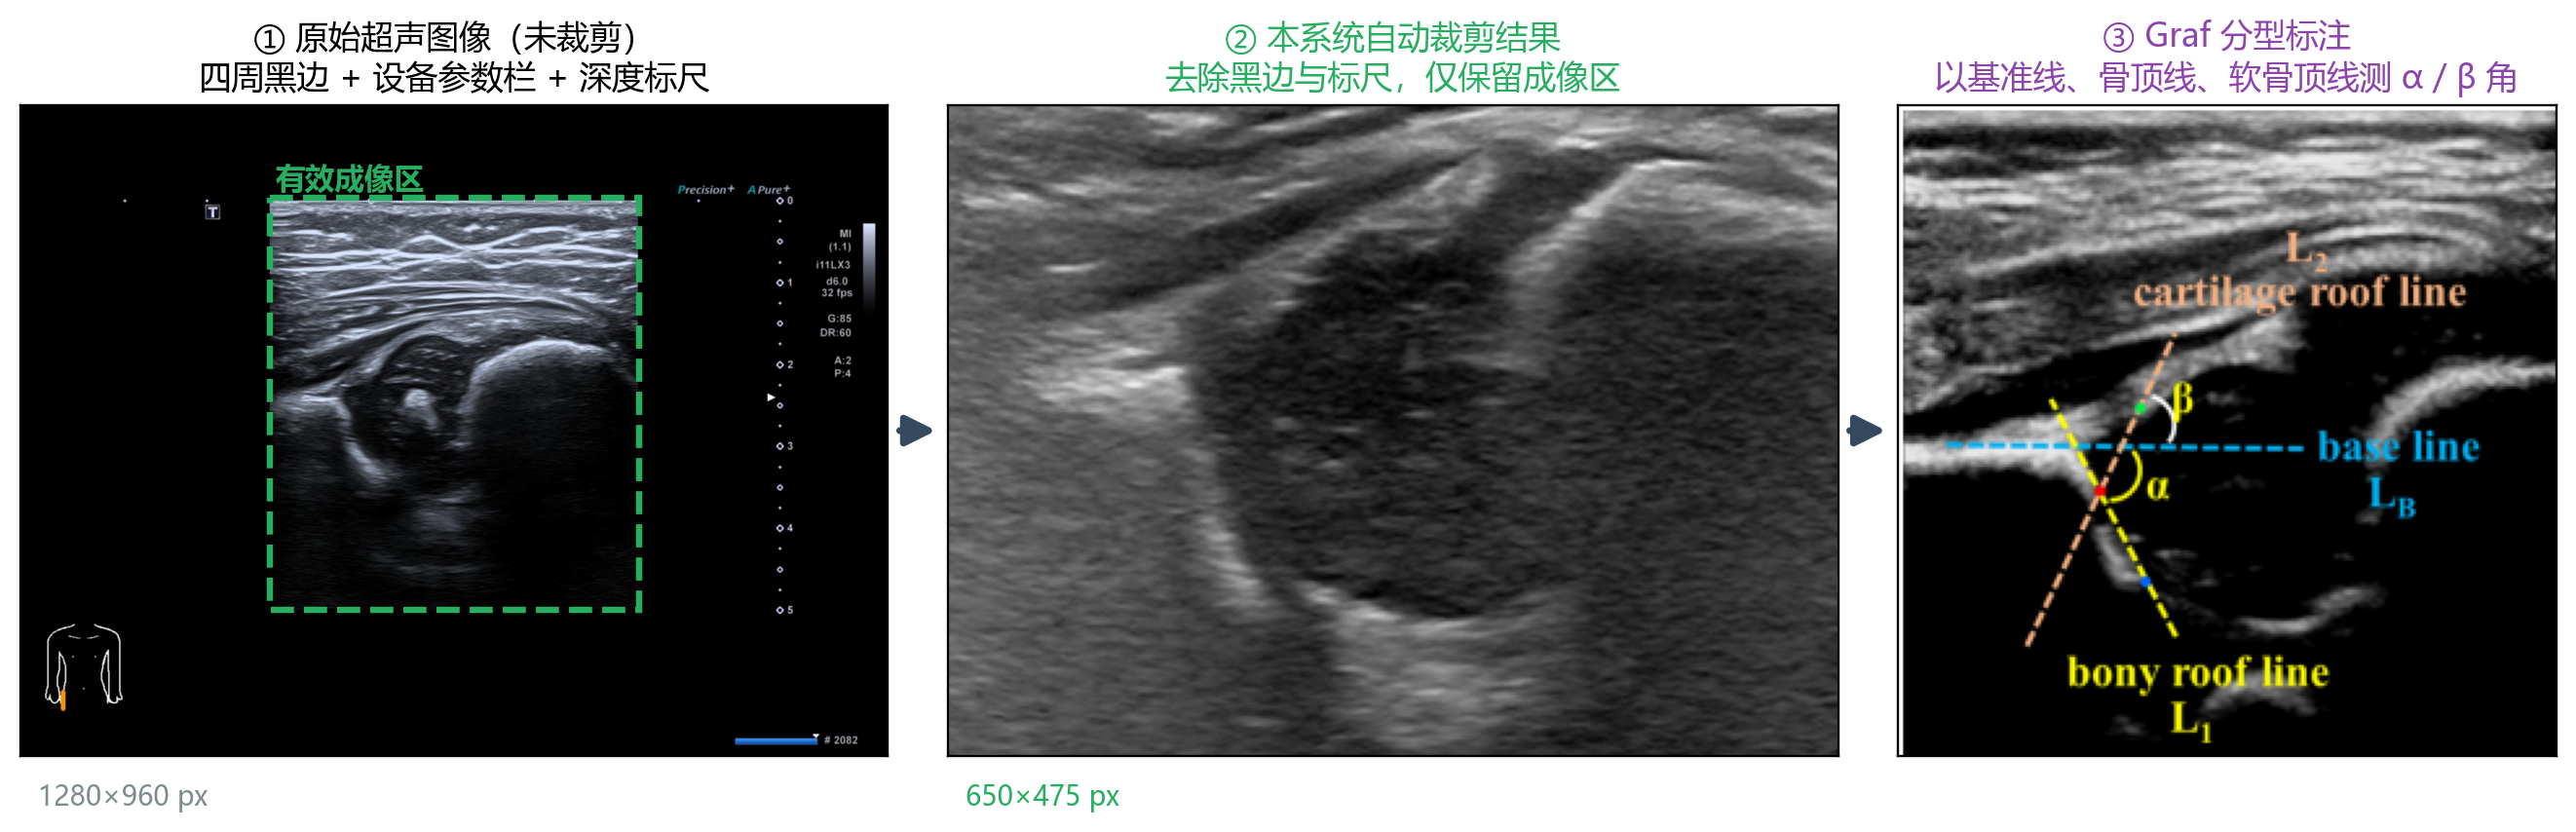
\includegraphics[width=0.94\textwidth]{fig_bg_compare.png}
\caption{设计目标：把 ①→② 这一步自动化，为 ③ 的 Graf 分型提供干净输入。左：设备导出的整屏截图；中：本系统自动裁剪结果；右：Graf 分型所需的三条标准线与 $\alpha$/$\beta$ 角——以基准线（base line, $L_B$）为参照，测量骨顶线（bony roof line, $L_1$）与软骨顶线（cartilage roof line, $L_2$）所夹锐角\cite{graf1984classification}}
\label{fig:bg}
\end{figure}

\noindent\textbf{本项目的定位很明确}：我们不解决 ③（Graf 分型诊断），我们解决 ①→② 这一步——\textbf{让进入分型环节的图像是干净、规范、口径一致的}。

\subsection{国内外研究现状：这一环节尚属空白}

为确认该环节是否已有成熟方案，我们系统检索了 DDH 领域的 AI 研究。Bhavsar 等 2025 年的系统综述纳入了 \textbf{23 项} DDH 人工智能研究\cite{bhavsar2025ddh}，其中 15 项针对髋关节超声（合计 8\,315 张）、8 项针对骨盆 X 线片（7\,091 张），报告 AUC 在 0.80--0.99 之间。这些工作集中在\textbf{分型、测角、标准切面识别}等下游任务上，\textbf{我们未检索到专门针对"成像区裁剪"这一前置环节的系统性工作}。该综述亦将"图像质量优化与自动化"列为未来方向。

{\small\itshape 注：此处表述为"未检索到"，而非"不存在"。检索范围限于 PubMed / Web of Science 主要索引中可获取的英文与中文文献。}

\subsection{设计目标}

基于上述背景，本项目确立三个层次的目标：

\begin{enumerate}[leftmargin=1.6em,itemsep=1.5pt,topsep=2pt]
\item \textbf{自动化}：把"从整屏截图裁出纯成像区"这一人工步骤，变为一次文件夹导入即可完成的自动流程；
\item \textbf{规范化}：所有图像采用统一的裁剪口径，消除人工之间的判断差异，为后续测角提供一致基准；
\item \textbf{轻量化}：在普通办公电脑（无独立显卡）上即可运行，单张耗时控制在秒级以下。
\end{enumerate}

\subsection{效率对比：量化人工与自动的差距}

为量化上述目标的实际价值，我们做了人工与本系统两组对照。

\noindent\textbf{人工裁剪}：本组 3 名成员，每人使用 Windows 自带"画图"软件手工裁剪 10 张，从打开第一张到全部保存完毕计时。三名被试的原始记录与单张平均如下：

\begin{center}\small
\begin{tabular}{cccc}
\toprule
被试 & 原始记录 & 折算秒 & 单张平均 \\
\midrule
第 1 人 & 2 分 34 秒 96 & 154.96 & 15.50 \\
第 2 人 & 2 分 20 秒 78 & 140.78 & 14.08 \\
第 3 人 & 2 分 43 秒 45 & 163.45 & 16.35 \\
\midrule
\multicolumn{2}{c}{人均} & \textbf{153.06} & \textbf{15.31} \\
\bottomrule
\end{tabular}
\captionof{table}{三名成员人工裁剪耗时（每人 10 张，Windows 画图）}
\end{center}

\noindent\textbf{本系统}：测试平台为\textbf{联想拯救者 Y7000P 笔记本}，搭载 Intel Core i7 处理器与 \textbf{NVIDIA GeForce RTX 4060 Laptop（8\,GB 显存）}，内存 16\,GB，运行 Windows 11，全程离线。端到端耗时（含黑边去除、窗口定位、边界预测与保存）实测 \textbf{CPU 199.31\,ms/张}、\textbf{GPU 66.93\,ms/张}。

\noindent 也就是说，人工一人的单张耗时（15.31\,s）相当于本系统 CPU 端 \textbf{77 张}的处理时间。按 400 张计，人工约需 \textbf{102 分钟}，本系统只需 \textbf{1.3 分钟}。

\begin{figure}[htbp]
\centering
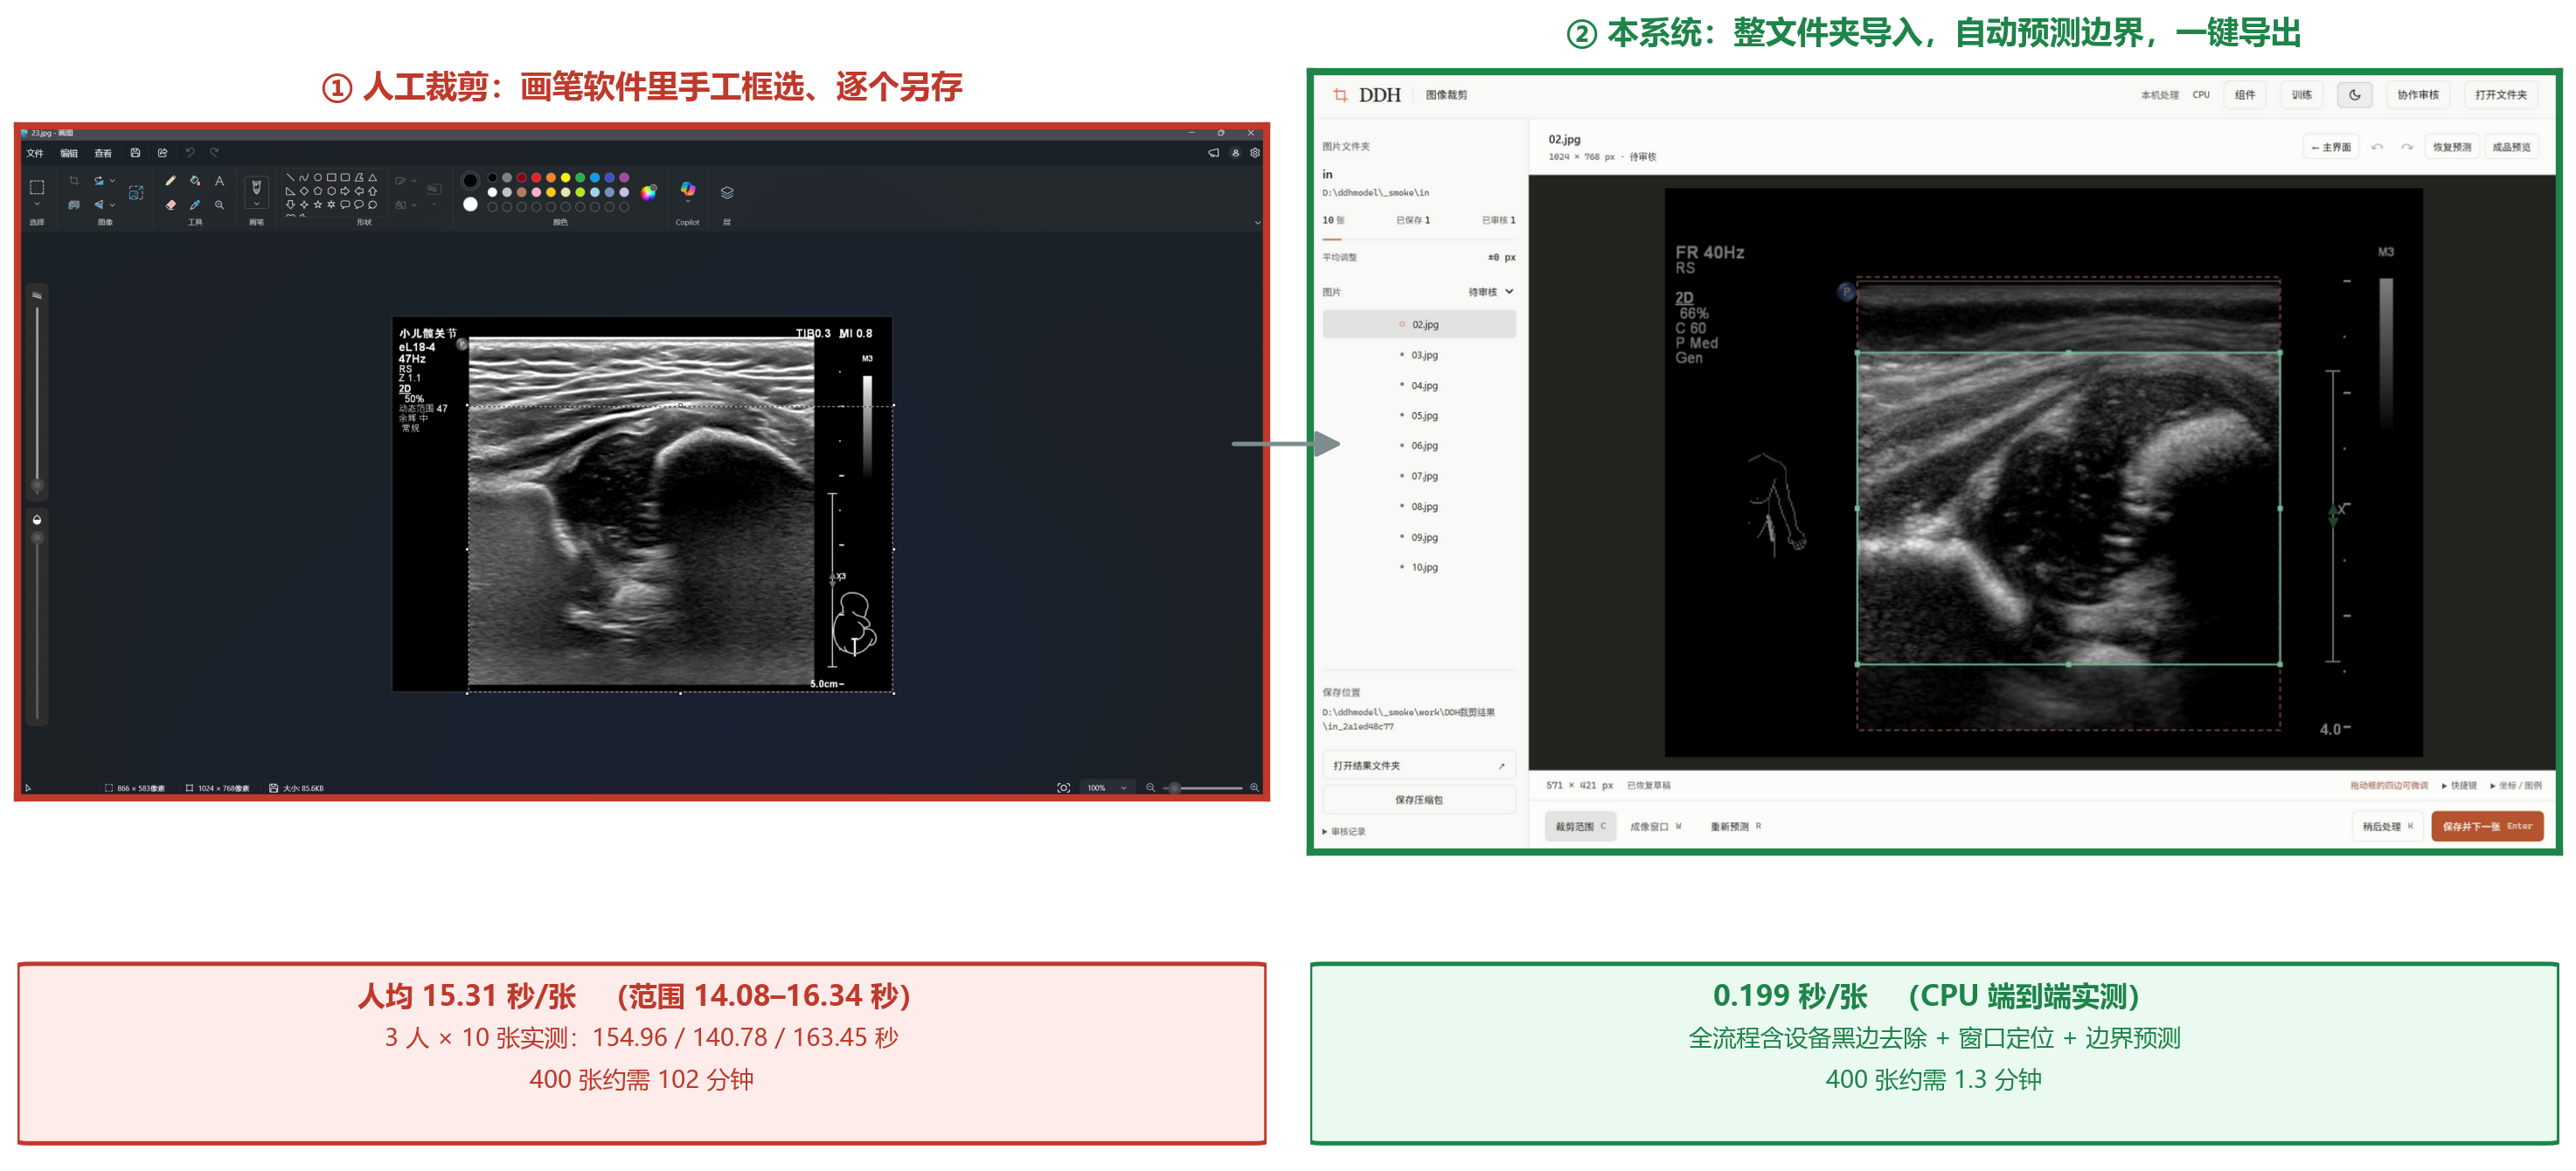
\includegraphics[width=0.82\textwidth]{fig_manual_vs_auto.png}
\caption{人工裁剪与本系统自动出图的效率对比。左为手工在"画图"软件中框选并逐个另存；右为本系统整文件夹导入、自动预测边界、一键导出}
\label{fig:manual}
\end{figure}

\noindent 值得注意的是，\textbf{人工耗时的主体并不在"拖框"本身}。在"画图"里拖出一个框通常不到 10 秒，真正把时间拉长的是\textbf{打开图片、保存结果、再去找下一张}这一整套操作——它们不涉及任何判断，却是逐张处理无法回避的部分。手工流程必须一张一张地重复这些步骤，而本系统的批量模式把它们整体消掉：\textbf{77 倍的差距不是来自"框得更快"，而是来自"不需要逐张框"}。
% ==================== 2 技术方案 ====================
\section{技术方案}

\subsection{总体设计思想：为什么是两阶段}

一个直觉的方案是"用一个检测网络直接框出成像区"。我们没有采用，原因在于\textbf{两类误差的量级完全不同}：

\begin{itemize}[leftmargin=1.6em,itemsep=1.5pt,topsep=2pt]
\item \textbf{左右边界}由黑边决定，几乎是确定的几何量——规则算法在 862 张老设备图像上"四边均 $\le4$\,px"的命中率为 94\%，在 89 张新设备图像上为 93\%（\textbf{此处"四边"指第一阶段输出的成像窗口四条边}，真值为人工确认的窗口；曾最费手的右边界在这 89 张上从改进前的 26\% 提升到 97\%，改进前中位偏差为偏宽 71\,px），\textbf{且无需任何训练数据}；
\item \textbf{上下边界}由组织回声决定，是模糊的语义量，必须靠学习。
\end{itemize}

\noindent 若把两者交给同一个网络，网络的容量会被"左右边界很好学"这一简单任务占据，反而削弱对上下边界的拟合能力。因此采用\textbf{分而治之}：规则负责确定性几何，网络负责模糊语义。这一范式与 Faster R-CNN 的"区域提议 + 框内细化"同构\cite{ren2015fasterrcnn}，也与近期 DDH 领域的标准切面识别工作思路一致\cite{ahn2025standardplane}。

\subsection{第一阶段：成像窗口定位}

\subsubsection{核心判据：为什么不用亮度阈值}

最直接的想法是用亮度阈值区分成像区与黑边。实测否定了这条路：\textbf{成像区内部存在大片无回声暗区}，其灰度均值与黑边接近（甚至为 0），亮度阈值会把它们判成黑边。

真正稳定可分的是\textbf{"是否纯黑"}——黑边像素恒等于 0，而成像区即使最暗处也总有相当比例的像素大于 $2/255$（实测深部暗区的非纯黑占比为 0.36--0.88）。判据取

\begin{equation}
\mathrm{content}(x,y)=\begin{cases}1, & I(x,y)>\tau_0,\\ 0, & \text{otherwise},\end{cases}\qquad \tau_0=2/255 .
\end{equation}

\noindent 为避免逐像素噪声，把二值图按 $4\times4$ 块聚合，块内非纯黑占比超过 $\tau_b=0.05$ 则该块记为内容。\textbf{必须先做像素级判定再聚合到块}：缩放会把暗区稀疏斑点平均掉，导致深部内容被误判为黑边——这正是早期版本的失败原因。

\subsubsection{五步流程与真实中间结果}

定位算法分五步，图~\ref{fig:window} 给出了\textbf{同一张截图的真实中间结果}，每一步都可肉眼核对：

\begin{enumerate}[leftmargin=1.6em,itemsep=1.2pt,topsep=2pt]
\item \textbf{块级内容掩膜}：按上述纯黑判据生成 $4\times4$ 块级二值图；
\item \textbf{水平开运算}（$r=1$）：要求一个块在左右各 1 块内都连续存在才保留，删除深度标尺刻度点、TGC 指示条这类 1--2 块宽的竖细结构；
\item \textbf{二维闭运算}（$r=2$）+ \textbf{连通域标记}：填补小块空洞，用两遍扫描加并查集取面积最大连通域的外接框；
\item \textbf{块坐标还原}：把粗框的 $4\times4$ 块坐标乘 4 换回像素坐标（\texttt{box = [x0*BLOCK, ...]}）；
\item \textbf{黑走廊判据 + 像素级梯度吸附}：\textbf{在上一步得到的像素坐标上}做走廊扫描与 $\pm12$\,px 吸附，把边界从块精度细化到像素精度（详见 2.2.3）；
\item \textbf{输出最终窗口}：得到纯成像区。
\end{enumerate}

\begin{figure}[htbp]
\centering
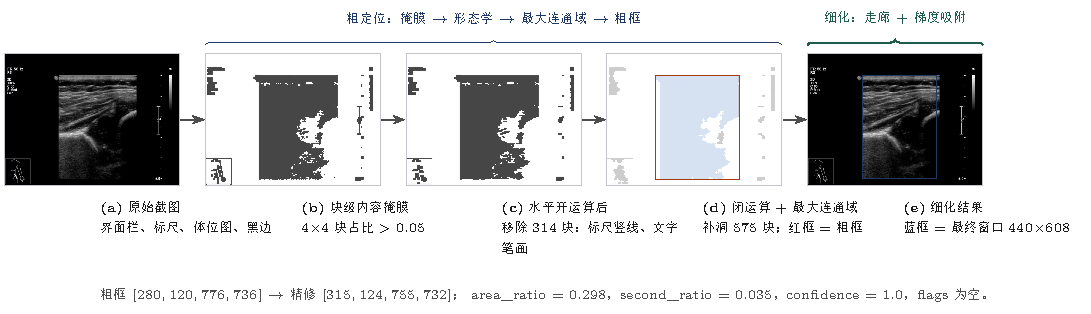
\includegraphics[width=0.9\textwidth]{fig3_window.pdf}
\caption{成像窗口定位全过程（真实中间结果，同一张截图）。(a) 原始截图；(b) 块级内容掩膜；(c) 水平开运算后，标尺竖线与文字笔画被移除 314 块；(d) 闭运算后补洞 575 块，浅蓝为最大连通域，红框为粗框；(e) 走廊判据与梯度吸附后的最终窗口}
\label{fig:window}
\end{figure}

\noindent\textbf{开运算必须在闭运算之前}。若顺序颠倒，稀疏的标尺点会先被膨胀成横贯的桥，把成像区与右侧界面连成一整块，之后再无法分开（实测最大连通域右边界会被拖到 $x=984$，而真实内容止于 $x=864$）。

\subsubsection{边界细化：黑走廊 + 像素级梯度吸附}

各型号设备的版式有一个共同结构：\textbf{成像内容 $\rightarrow$ 一条黑走廊（窗外）$\rightarrow$ 才是界面元素}。由此可以只判断"边在哪"，而不必把"内容"与"界面"用阈值分开。

算法从内容内部（占用率最高的一列）向两侧逐列扫描，遇到\textbf{连续 $\geqslant2$ 列占用率低于 $\tau_{\mathrm{low}}=0.35$} 即判定进入走廊，该处为粗边界；再在 $\pm12$\,px 邻域内，以"跨边界两侧各 4\,px 的平均占用率之差最大"为准做\textbf{像素级吸附}。

\begin{figure}[htbp]
\centering
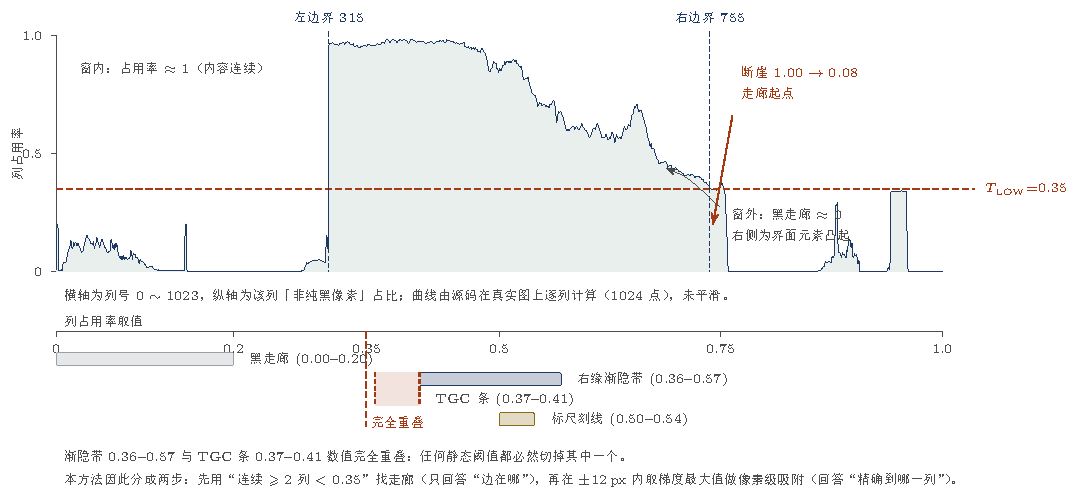
\includegraphics[width=0.80\textwidth]{fig4_corridor.pdf}
\caption{走廊判据的必要性。上：真实截图的逐列占用率剖面（1024 个采样点），窗内平台 $\approx1$、边界断崖、窗外走廊 $\approx0$；下：窗口右缘渐隐带与 TGC 条的取值区间完全重叠，静态阈值必然误伤其一}
\label{fig:corridor}
\end{figure}

\noindent 之所以必须分层，是因为\textbf{任何静态阈值都分不开两者}：老设备窗口右缘本身是渐隐的（占用率 0.36--0.57），与 TGC 条（0.37--0.41）数值完全重叠，如图~\ref{fig:corridor} 下半部分所示。走廊法把界面元素挡在走廊之外，只负责"边在哪"；吸附负责"精确到哪一列"。扫描前还需对剖面做 \textbf{3 列中值滤波}：走廊里常夹着标尺短横这类单列亮点，会打断"连续低列"计数，使走廊起点晚判 5--8\,px；而内容断崖处（$1.00\to0.08$）中值几乎不动。

\subsubsection{上下边界、参数标定与拒识}

上下边界改为\textbf{从粗框外缘向内扫描}，取第一条非纯黑占比超过 $\tau_e=0.20$ 的行。方向很关键：窗口底部有一条很暗的窄带（行灰度仅 0.6--7.8），若从内容深处向外游走会被它截断；而窗外文字行的占用率只有 0.03--0.08，低于阈值不会被误选。全部关键参数见表\ref{tab:params}。

\begin{center}\small
\begin{tabular}{llc}
\toprule
参数 & 作用 & 取值 \\
\midrule
$\tau_0$ & 像素级纯黑判据 & $2/255$ \\
$\tau_b$ & 块级内容占比阈值 & 0.05 \\
$\tau_{\mathrm{low}}$ & 走廊判据：连续低列阈值 & 0.35 \\
$\tau_e$ & 行级端点判据 & 0.20 \\
中值滤波窗 & 抑制标尺单列亮点 & 3 列 \\
吸附搜索半径 & 像素级边界细化 & $\pm12$\,px \\
\bottomrule
\end{tabular}\\[2pt]
\captionof{table}{窗口定位的关键参数（均由实测标定）}\label{tab:params}
\end{center}

\noindent\textbf{拒识机制}：面积占比越界（$<5\%$ 或 $>95\%$）、第二大连通域超过最大域的 25\%（拼图/双屏）、窗口贴图像边界，均标记为可疑；窗口之外若仍有一整片实心内容（占用率 $>0.5$ 且连续 5 块），追加 \texttt{content\_beyond\_*} 标记。\textbf{系统宁可标记可疑，也不静默输出错误裁剪}。

\subsection{第二阶段：CropNet 边界回归}

\subsubsection{输入预处理与网络结构}

窗口裁出的图像长宽比悬殊，而网络要求固定输入。若直接拉伸，解剖结构会变形、边界位置随之偏移；因此采用 \textbf{letterbox}：按 $s=\min(384/w,384/h)$ 等比缩放后居中补黑，同时记录真实内容在 $384\times384$ 画布中的位置 $[p_x,p_y,p_x{+}n_w,p_y{+}n_h]$，供后续 ROIAlign 使用。

\begin{figure}[htbp]
\centering
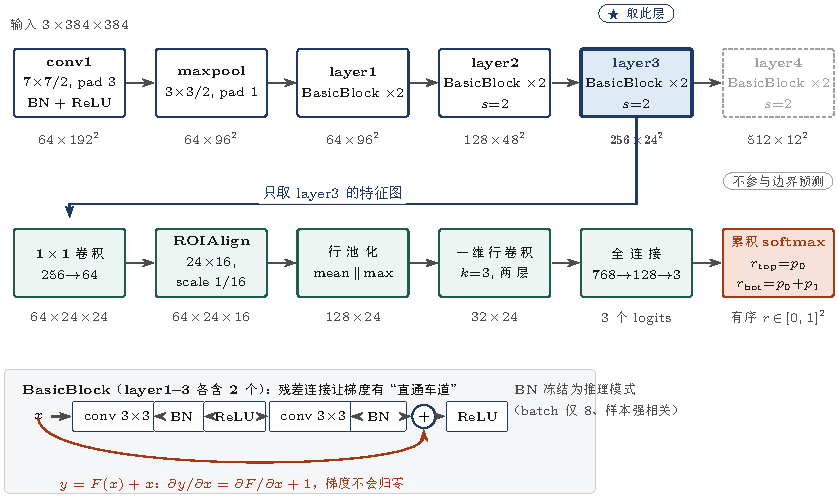
\includegraphics[width=0.86\textwidth]{fig5_cropnet.pdf}
\caption{CropNet 结构与张量形状。主干逐级降采样至 layer3 的 $256\times24\times24$；边界分支经 $1\times1$ 投影、ROIAlign\cite{he2017maskrcnn}、行池化、一维行卷积与全连接输出三个 logits。左下为 BasicBlock 的残差结构}
\label{fig:cropnet}
\end{figure}

\subsubsection{为什么取 Layer3：感受野与分辨率的折中}

主干采用 ImageNet 预训练的 ResNet-18\cite{he2016resnet}，\textbf{只取到 layer3}，其 $256\times24\times24$ 的特征图进入边界分支。

这一取舍由两个约束共同决定：\textbf{要定位的是"第几行"，既要求看得见足够上下文，又要求分辨率够细}。按感受野递推实测（只计主干支路）：Layer1 为 43\,px、Layer2 为 99\,px、Layer3 为 211\,px、Layer4 为 435\,px——\textbf{只有 Layer4 超过输入高度 384\,px}；但 Layer4 的纵向只有 12 格，一格代表 32\,px，边界会明显跳变，而 Layer3 纵向 24 格、一格 16\,px。\textbf{实测 Layer3 与 Layer4 的定位精度无显著差异（$p=0.8678$），因此在"分辨率更细、算力更低"的一侧选 Layer3：再深一层牺牲分辨率，再浅一层语义不足，$24\times24$ 是折中点。}

\subsubsection{多层级融合：理论上更优的下一步}

一个自然的追问是：\textbf{只取 layer3 是否浪费了浅层信息？}

理论上，\textbf{融合 Layer1+2+3 更合理}。Layer3 的 $24\times24$ 特征图上纵向一格为 16\,px，对边界定位偏粗；而 Layer1 输出 $96\times96$（总步幅 4），一格为 4\,px，保留了更细的纵向位置信息；把浅层的精细位置与深层的抽象语义结合，理论上应优于单层。这一推断有实验支撑但\textbf{未达统计显著}：在 \textbf{ResNet-18 上，L1+2+3 融合把 3\% 容差合格率从 51.1\% 提升到 56.8\%（+5.7 个百分点，McNemar $p=0.3323$）}，上边界均值从 17.39\,px 降到 16.97\,px（$p=0.8908$）——\textbf{方向一致向好，但幅度在噪声范围内}。

需要如实说明的是：该提升在当前 88 张测试集上\textbf{未达统计显著}（上边界 $p=0.89$，合格率 McNemar $p=0.33$）。因此目前\textbf{生产环境部署的仍是单层 layer3 模型}，融合版本作为已验证的候选方案，将在扩大测试集后重新评估——若后续数据证实，可直接替换，无需改动系统其他部分。

\subsubsection{行向量化与一维行卷积}

上下边界只与"行"有关，宽度方向是干扰，因此先用 ROIAlign 把真实内容区域双线性采样成固定 $24\times16$ 网格——相比 RoIPool 的量化取整，ROIAlign 用浮点坐标插值，无像素级错位。随后对每一行的 16 个值分别取均值与最大值，拼接成 128 维行向量：

\begin{equation}
\mathbf{r}_j=\big[\,\mathrm{mean}_{c}\mathbf{F}[c,j,:]\;\big\|\;\max_{c}\mathbf{F}[c,j,:]\,\big]\in\mathbb{R}^{128},\qquad j=1,\dots,24 .
\end{equation}

\noindent 均值反映整体强度、最大值保留强响应，两者互补。接下来沿高度方向做一维卷积，让相邻行互相参考：

\begin{equation}
\mathbf{y}_j=\mathrm{ReLU}\Big(\sum_{\delta=-1}^{+1}\mathbf{W}_\delta\,\mathbf{r}_{j+\delta}+\mathbf{b}\Big),\qquad k=3,\ \texttt{padding}=1 .
\end{equation}

\noindent $k=3$、padding$=1$ 保证输出长度仍为 24，两层堆叠后感受野从 3 行扩到 5 行（图~\ref{fig:rowconv}）。关键在于：判断第 $j$ 行是否为边界，不能只看第 $j$ 行，而要看第 $j-1$ 至 $j+1$ 行的上下文；一维卷积只在行序列上滑动，\textbf{不会像二维卷积那样同时混入宽度方向的信息}。输出 $32\times24$ 展平为 768 维送入全连接头。

\begin{figure}[htbp]
\centering
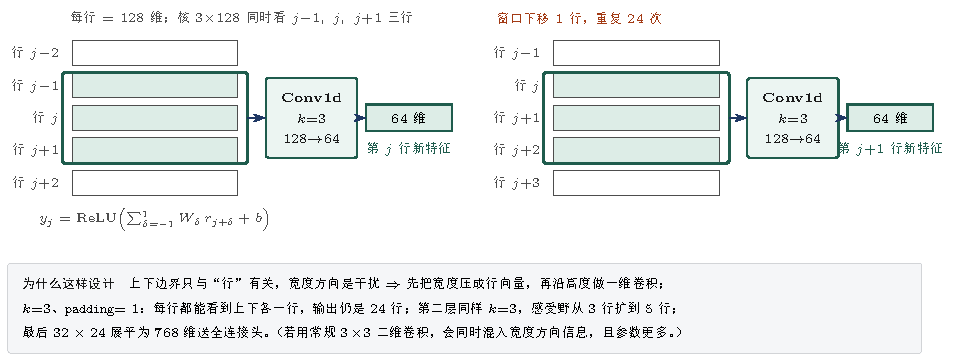
\includegraphics[width=0.80\textwidth]{fig7_rowconv.pdf}
\caption{一维行卷积的逐行计算过程。左：计算第 $j$ 行时卷积核覆盖第 $j-1$、$j$、$j+1$ 行；右：窗口下移一行，输出第 $j+1$ 行的新特征}
\label{fig:rowconv}
\end{figure}

\subsubsection{累积 softmax：有序性由结构保证}

若直接回归 $(\hat r_{\mathrm{top}},\hat r_{\mathrm{bot}})$，训练早期极易输出上下颠倒的非法解，只能靠额外损失项纠正。本文改为输出 3 个 logits，softmax 得到三段概率后\textbf{累积求和}：

\begin{equation}
p=(1-3\times10^{-4})\cdot\mathrm{softmax}(\mathbf{z})+10^{-4},\qquad
\hat r_{\mathrm{top}}=p_0,\quad \hat r_{\mathrm{bot}}=p_0+p_1 ,
\end{equation}
\begin{equation}
\hat r_{\mathrm{bot}}-\hat r_{\mathrm{top}}=(p_0+p_1)-p_0=p_1\geqslant10^{-4}>0 .
\end{equation}

\noindent 几何上，把窗口高度视为 $0\sim1$ 的线段，三段正好分成"上空白 / 保留区 / 下空白"。由于 softmax 各项非负、且整体又加了 $10^{-4}$ 的平滑下界，故 $p_1\geqslant10^{-4}>0$ 严格成立，$\hat r_{\mathrm{top}}<\hat r_{\mathrm{bot}}$ \textbf{恒成立}——上下顺序由输出结构保证，而非靠损失惩罚出来。

\begin{figure}[htbp]
\centering
\begin{minipage}[t]{0.52\textwidth}
\centering
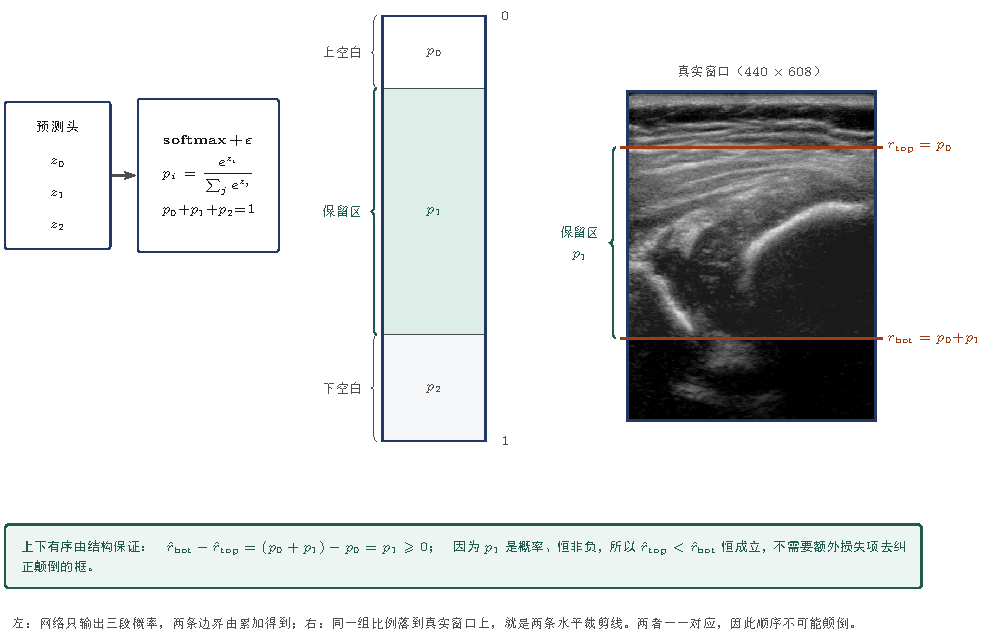
\includegraphics[width=\textwidth]{fig8_ordered.pdf}
\par\vspace{2pt}
\parbox{0.96\textwidth}{\footnotesize (a) 累积 softmax：有序性由结构保证。网络只输出三段概率，两条边界由累加得到}
\end{minipage}\hfill
\begin{minipage}[t]{0.44\textwidth}
\centering
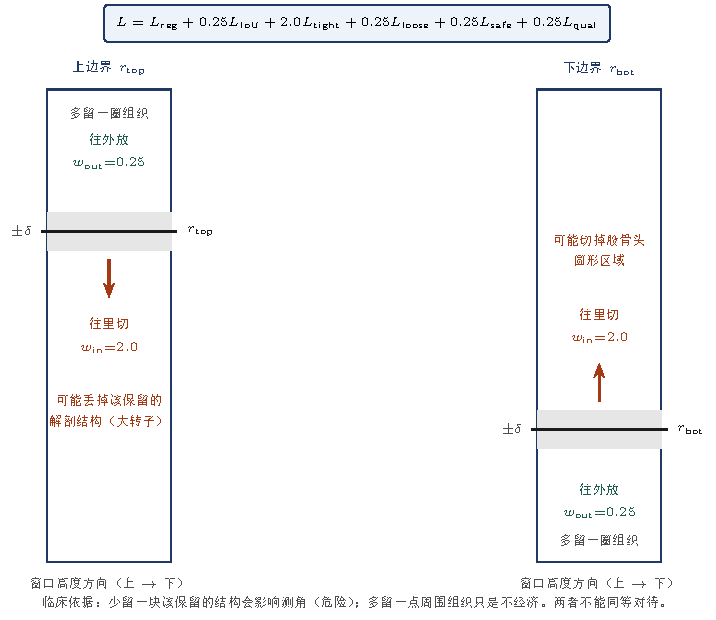
\includegraphics[width=\textwidth]{fig9_loss.pdf}
\par\vspace{2pt}
\parbox{0.96\textwidth}{\footnotesize (b) 非对称损失：向内过裁的惩罚是向外欠裁的 8 倍}
\end{minipage}
\caption{两处"把约束写进结构"的设计。(a) 累积 softmax 使上边界必然小于下边界，顺序不可能颠倒；(b) 容差带之外，往内裁与往外裁被赋予 8 倍惩罚差，把"宁可多留不可切掉"的临床直觉变成可优化的数学目标}
\label{fig:ordered}
\end{figure}
\noindent 这一改动的收益在训练早期最明显：直接回归时前几个 epoch 有相当比例样本输出非法框，梯度方向被这些样本带偏；改成累积 softmax 后，非法框从结构上不再可能出现，损失曲线也更平滑，省掉了"额外加一项惩罚"的调参工作。

\subsubsection{非对称损失：把临床优先级编码进目标函数}

临床上，把边界往\textbf{内}裁（少留、切掉该保留的成像区结构）比往\textbf{外}留（多留一圈周围组织或黑边）严重得多：\textbf{少留一块该保留的结构会影响测角，多留一圈只是不经济}。为此对两个方向分别按不同权重惩罚，且\textbf{容差带之内不惩罚}。记标注上、下边界为 $\ell_{\text{top}},\ell_{\text{bot}}$，预测为 $\hat r_{\text{top}},\hat r_{\text{bot}}$，容差 $\delta$（取窗口高度的 4\%），则

\begin{equation}
\begin{aligned}
\mathcal{L}_{\text{asym}} = \frac{1}{N}\sum_{i}\Big[&\;
w_{\text{in}}\cdot\big(\max(0,\hat r_{\text{top}}-\ell_{\text{top}}-\delta)+\max(0,\ell_{\text{bot}}-\delta-\hat r_{\text{bot}})\big)\\
+\;& w_{\text{out}}\cdot\big(\max(0,\ell_{\text{top}}-\delta-\hat r_{\text{top}})+\max(0,\hat r_{\text{bot}}-\ell_{\text{bot}}-\delta)\big)\Big],
\end{aligned}
\end{equation}

\noindent 第一行两项是\textbf{向内过裁}（上边界往下切、下边界往上切），第二行两项是\textbf{向外欠裁}。

\noindent 其中 $w_{\text{in}}=2.0$、$w_{\text{out}}=0.25$。\textbf{关键在于这两个方向是靠 $(\hat r-\ell)$ 的符号区分出来的，不是在同一个绝对误差上加分段权重}：$\delta$ 之内的偏差被 $\max(0,\cdot)$ 截成 0，因此\textbf{落在容差带内的样本损失恰为 0}；只有越过容差带、且方向不同时才分别计入。图示满窗高度 1、$\delta=0.04$ 时，\textbf{向内过裁 0.11 产生损失 0.44，向外欠裁同样 0.11 只产生 0.055——相差 8 倍}。\textbf{这把"宁可多留一点黑边，也不能切掉成像区"的临床直觉，变成了可优化的目标函数}。

% ==================== 3 系统实现 ====================
\section{系统实现}

本系统以\textbf{Windows 离线客户端}形式交付，不依赖网络、不上传任何患者图像——这对医疗数据合规很关键。设计目标很朴素：\textbf{让前面两章的算法能被真正用起来}。

\subsection{主干功能与界面}

\begin{figure}[htbp]
\centering
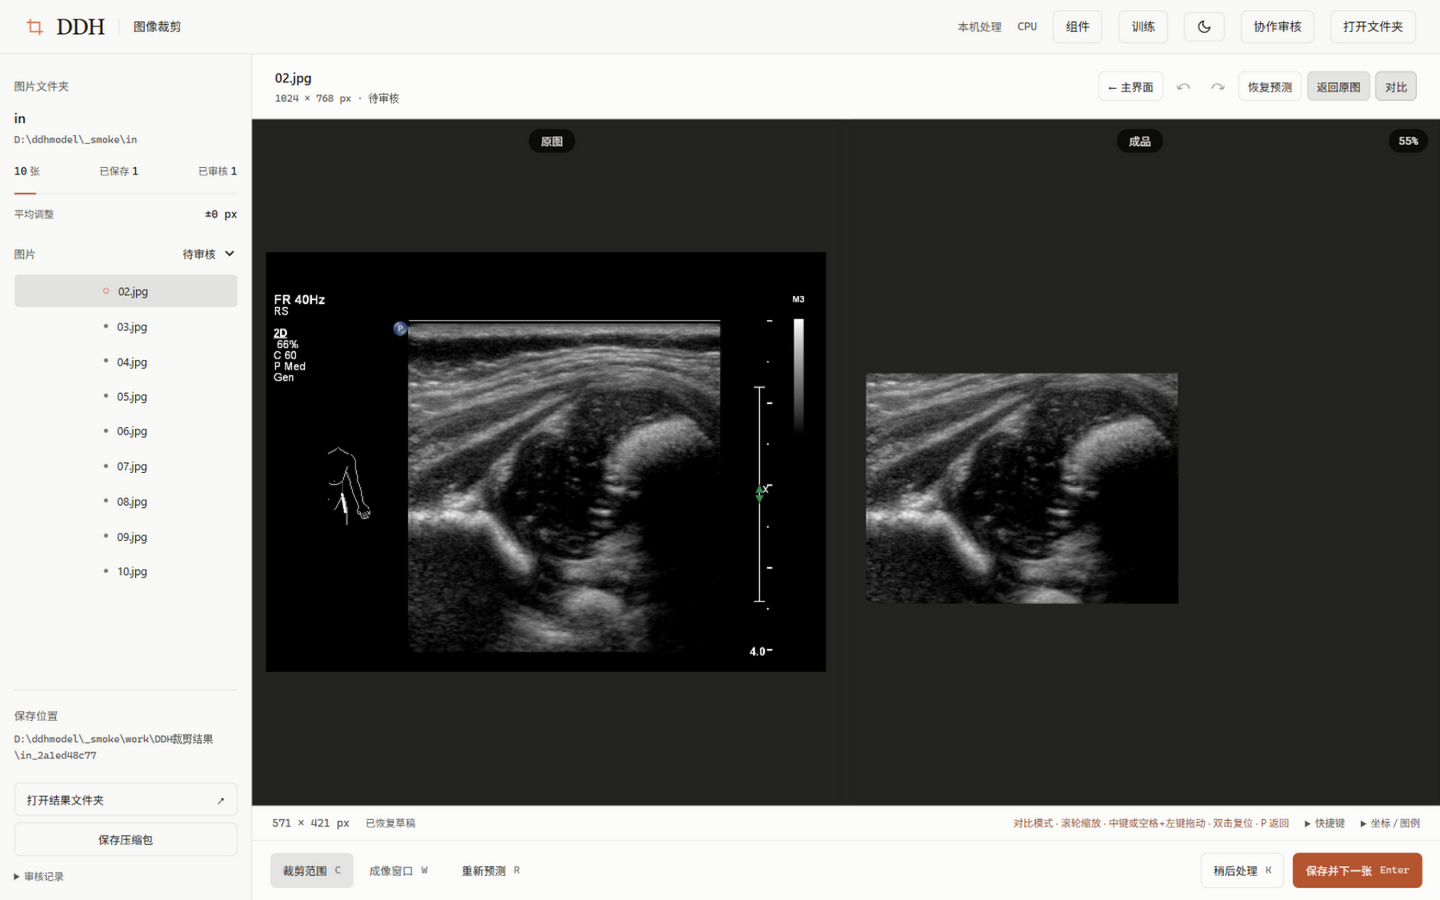
\includegraphics[width=0.62\textwidth]{fig_ui_preview.png}
\caption{客户端主界面（预览对比模式）。左侧为文件夹清单与批量进度，中部左为原图、右为裁剪成品，右侧为一键导出}
\label{fig:ui}
\end{figure}

\noindent 界面围绕"批量、可见、可干预"三个原则，对应三项主干功能：\textbf{批量导入导出}（一次导入整个文件夹，结果按原文件名自动保存，这是 77 倍提速真正兑现的地方）、\textbf{并排预览}（原图与成品同屏对照，预测边界直接画在图上）、\textbf{人工可干预}（可拖动边界、重设窗口、恢复预测或标记"稍后处理"——\textbf{人在回路，但工作量从"全做"降为"核对"}）。

\subsection{两种工作模式}

系统提供\textbf{逐张审核}与\textbf{批量直出}两种模式：前者适用于构建标注数据集与疑难样本，每张确认后可微调边界；后者适用于已有大批量图像、模型已可信的场景，一键处理整个文件夹。两者单张耗时不同——\textbf{逐张审核}约 1--1.5\,s/张，\textbf{批量直出}约 0.2\,s/张。第 1.5 节报告的 77 倍提速对应\textbf{批量直出}；若采用逐张审核模式，提速约为 10--15 倍，这一点如实说明。

\subsection{数据闭环}

\begin{figure}[htbp]
\centering
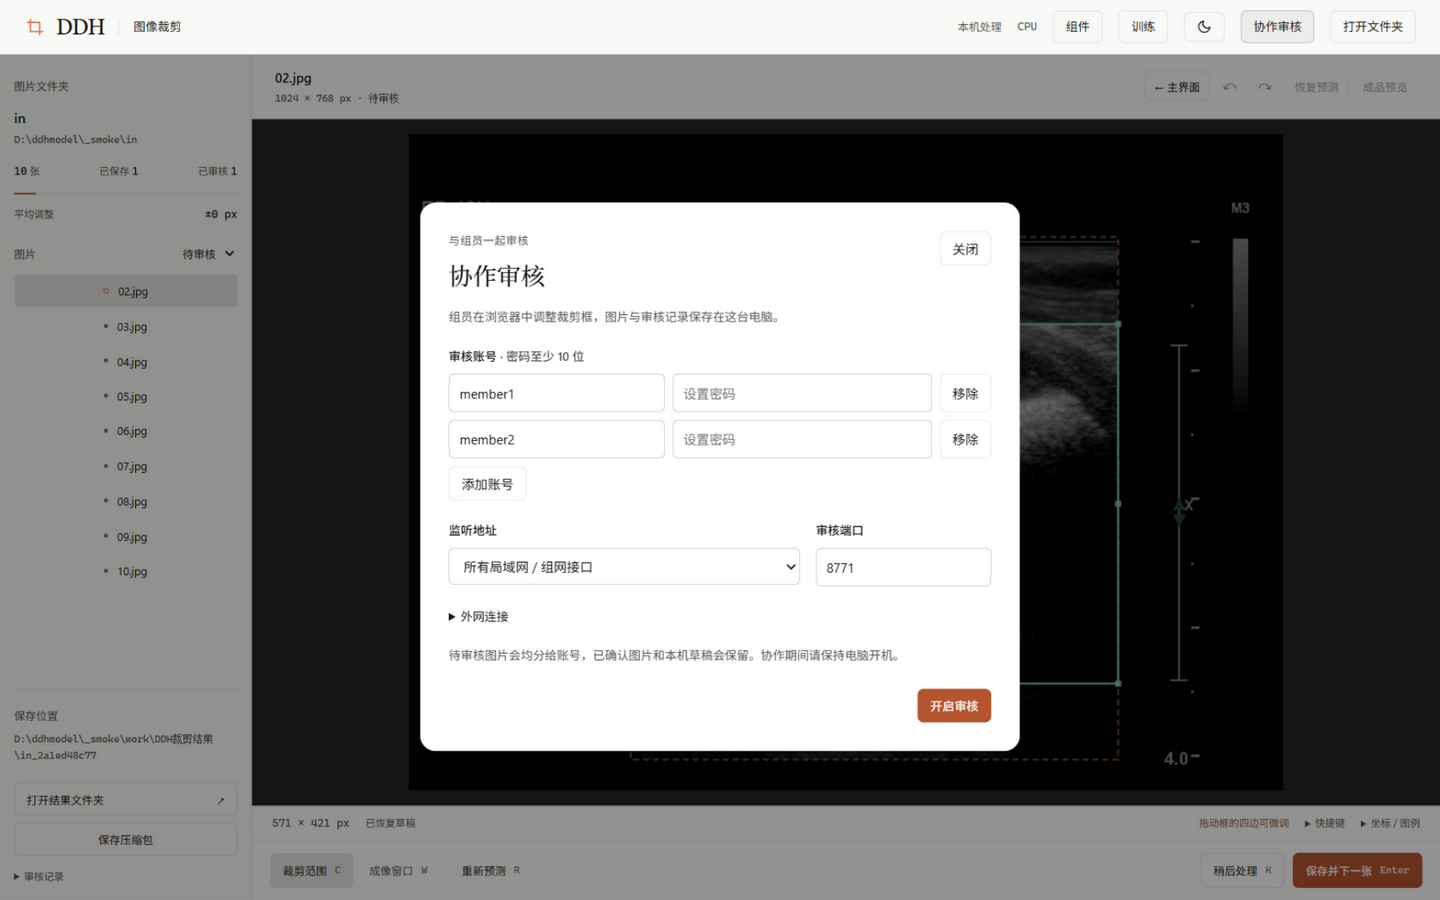
\includegraphics[width=0.52\textwidth]{fig_ui_review.png}
\caption{协作审核界面。裁剪结果可被多人复核、标记与留痕，形成"标注—训练—复核"的数据闭环}
\label{fig:review}
\end{figure}

\noindent 系统记录每张图的处理痕迹（谁审、何时、是否修改边界）。这一机制的价值不只在质量控制：\textbf{人工修正的结果可直接回流为新的训练样本}。第 5.5 节已表明标注质量是当前突破方向，而这套闭环正是持续提升标注质量的基础设施。
% ==================== 4 研究方法 ====================
\section{研究方法}

\subsection{数据集与评价指标}

\textbf{数据}：项目累计标注 1\,550 张真实超声图像（老批次 862 张 + 三成员新标注 688 张），覆盖三种设备型号。\textbf{本节 6 组配置的对照实验在其中的 862 张老批次图像上完成}——该子集标注口径与窗口标签统一，按 560 / 128 / 86 / 88 划分为训练/验证/校准/测试集，并\textbf{固定划分、固定随机种子（seed=42）}以保证所有配置可比。

\textbf{指标}：
\begin{itemize}[leftmargin=1.6em,itemsep=1.2pt,topsep=2pt]
\item 上下边界误差（像素，越小越好）；
\item 纵向 IoU（上下边界区间的重合度，越大越好）；
\item 容差合格率（误差在窗口高度 2\%/3\%/5\% 以内的比例）。
\end{itemize}

\subsection{选型的双重依据：文献 + 自证实验}

模型选型不能只凭"大的应该更好"的直觉。我们采用\textbf{外部文献 + 自有实验}的双重论证。

\subsubsection{外部依据：同类任务上 ResNet-50 的收益是边际的}

Lawley 等 2024 年在\textbf{超声}图像上系统对比了 9 种网络（含 ResNet-18/34/50/101/152），每种训练 20 次取最优\cite{lawley2024network}。

其中 ResNet-18 与 ResNet-50 的对照最有参考价值：参数量分别为 1118 万与 2354 万（\textbf{2.1 倍}），在完整数据 + 迁移学习下精度为 83.04\% 与 83.48\%——\textbf{仅差 0.44 个百分点}；而在小样本（800 张）下为 67.41\% 与 73.21\%（差 5.80 个百分点）。\textbf{数据越少，模型容量的差异反而越明显}。

\noindent 该文的核心结论是：\textbf{"数据集规模对精度的影响比网络选择更重要"}（\textit{Dataset size proved a more important factor in determining accuracy than network selection}）。

\noindent 对我们的启示很直接：\textbf{当参数量翻倍只换来 0.44 个百分点的提升时，是否值得为它付出 2 倍的训练与推理成本，取决于本任务能否测出这 0.44}。这必须由实验回答。

\subsubsection{自有实验：6 组同条件对照}

我们在\textbf{同一测试集（88 张）、同一划分、同一随机种子}上训练并评估了 6 组配置，覆盖两个维度：

\begin{center}\small
\begin{tabular}{llcc}
\toprule
编号 & 配置 & 主干 & 特征使用 \\
\midrule
A1 & \texttt{r18\_l3} & ResNet-18 & 仅 Layer3 \\
A2 & \texttt{r50\_l3} & ResNet-50 & 仅 Layer3 \\
B1 & \texttt{r18\_l123} & ResNet-18 & Layer1+2+3 融合 \\
B2 & \texttt{r50\_l123} & ResNet-50 & Layer1+2+3 融合 \\
C1 & \texttt{r18\_l4} & ResNet-18 & 仅 Layer4 \\
C2 & \texttt{r18\_l1234} & ResNet-18 & Layer1+2+3+4 融合 \\
\bottomrule
\end{tabular}
\captionof{table}{6 组对照实验的配置设置}
\end{center}

\noindent\textbf{统计方法}：对每一组对比做\textbf{配对 Wilcoxon 符号秩检验}（$n=88$ 张测试图，逐图配对），并以 5\,000 次配对 bootstrap 给出 95\% 置信区间。选择配对检验是因为同一张图在不同配置下的误差并非独立——配对能消除图像难度差异带来的方差。


% ==================== 5 实验结果与讨论 ====================
\section{实验结果与讨论}

\subsection{主结果：6 组配置的精度对比}

\begin{figure}[htbp]
\centering
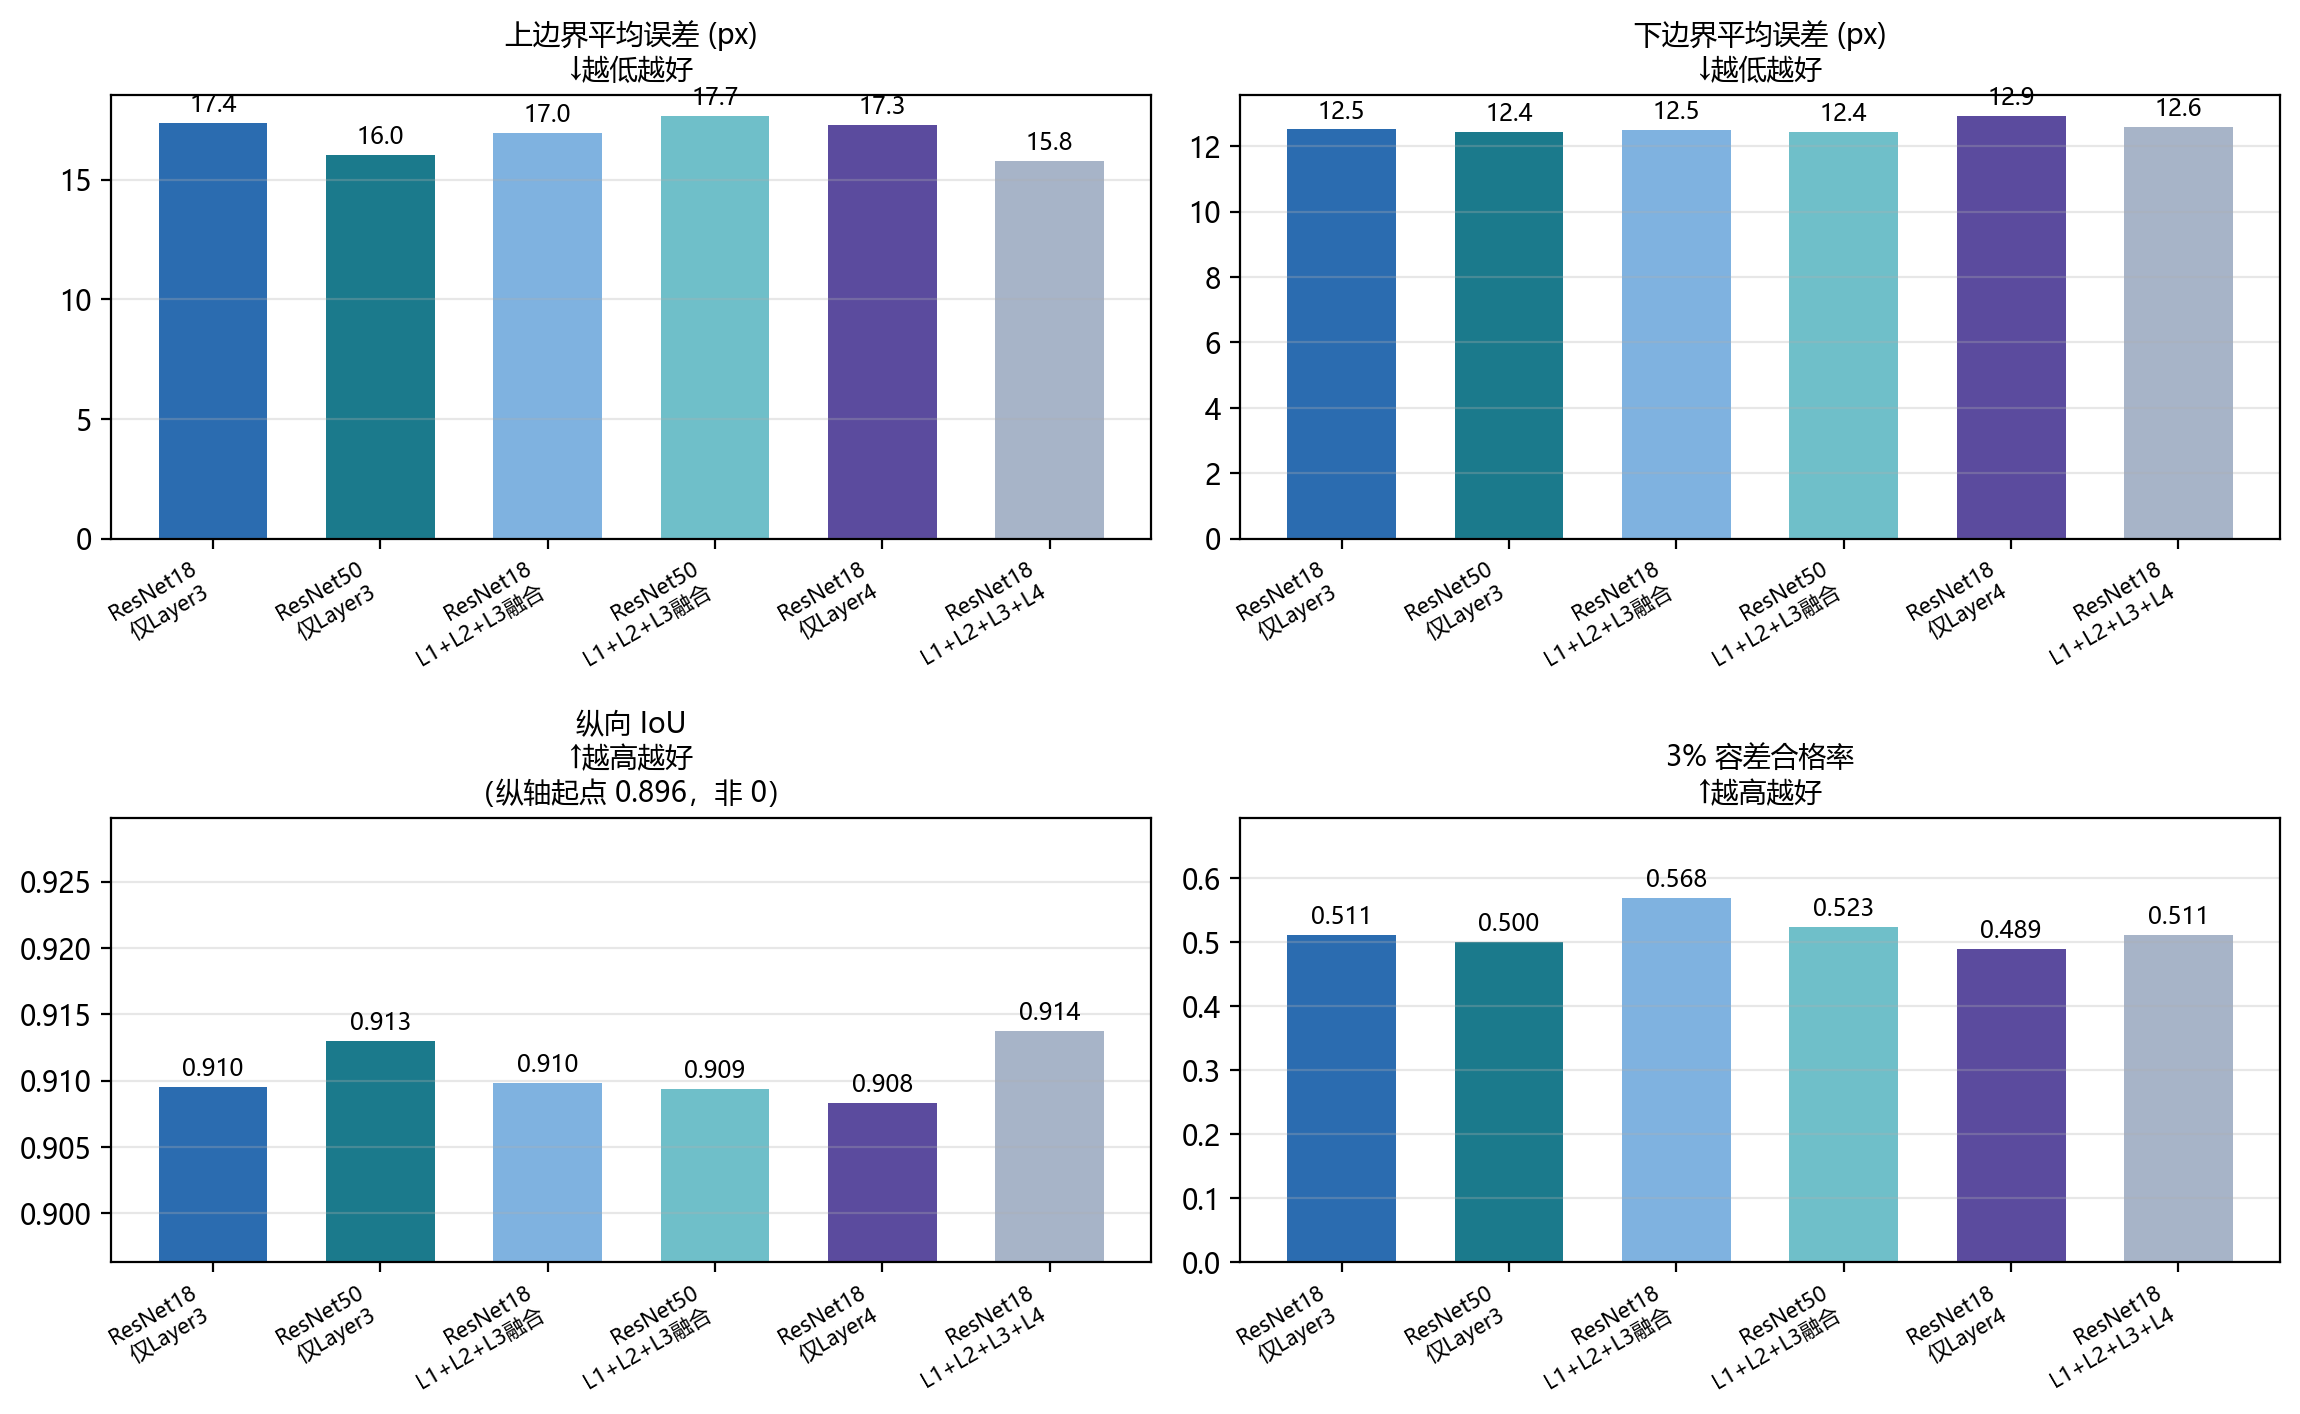
\includegraphics[width=0.74\textwidth]{fig3_main_metrics_bar.png}
\caption{6 组配置在同一测试集（88 张）上的裁剪精度对比}
\label{fig:main}
\end{figure}

\begin{table}[htbp]
\centering\small
\caption{6 组配置的精度与成本汇总（测试集 88 张）}
\label{tab:summary}
\begin{tabular}{lccccccc}
\toprule
配置 & 上边界均值 & 下边界均值 & 纵向 IoU & 3\% 合格率 & 参数量 & 模型大小 & CPU 推理 \\
     & (px) & (px) & & & (M) & (MB) & (ms) \\
\midrule
r18\_l3   & 17.39 & 12.51 & 0.9096 & 51.1\% & 11.37 & 43.5 & 30.7 \\
r50\_l3   & 16.03 & 12.44 & 0.9130 & 50.0\% & 23.75 & 90.9 & 78.5 \\
r18\_l123 & 16.97 & 12.50 & 0.9098 & 56.8\% & 11.41 & 43.6 & 33.2 \\
r50\_l123 & 17.66 & 12.44 & 0.9094 & 52.3\% & 23.88 & 91.4 & 81.6 \\
r18\_l4   & 17.30 & 12.92 & 0.9083 & 48.9\% & 11.41 & 43.6 & 31.7 \\
r18\_l1234& 15.77 & 12.59 & 0.9138 & 51.1\% & 11.45 & 43.8 & 33.9 \\
\bottomrule
\end{tabular}
\end{table}

\noindent 表面上看，不同配置之间的数字确有差异。但\textbf{统计检验表明这些差异绝大多数不显著}。

\subsection{关键发现一：换主干、加深层都没有显著收益}

\begin{center}\small
\begin{tabular}{lccccl}
\toprule
对比 & 上边界 $p$ & 下边界 $p$ & IoU $p$ & 3\% 合格率 $p$ & 结论 \\
\midrule
ResNet-18 vs 50（仅 L3） & 0.0805 & 0.9469 & 0.2165 & 1.0000 & 均不显著 \\
ResNet-18：L3 vs 融合 & 0.8908 & 0.8842 & 0.9635 & 0.3323 & 均不显著 \\
ResNet-50：L3 vs 融合 & \textbf{0.0398} & 0.7582 & 0.3002 & 0.8036 & 未校正负向 \\
ResNet-18：L123 vs L1234 & 0.0912 & 0.6264 & -- & -- & 不显著 \\
\bottomrule
\end{tabular}
\captionof{table}{四组配对 Wilcoxon 符号秩检验结果（$n=88$）}
\end{center}

\noindent 四组对比中，按 $4\times2$ 共 8 次比较做 Bonferroni 校正（$\alpha/8 = 0.00625$）后\textbf{没有任何一项达到显著}；未校正的名义水平下只有一项低于 0.05，且是\textbf{负向}的：在 ResNet-50 上启用多尺度融合，上边界误差从 16.03\,px 增加到 17.66\,px（$p=0.0398$，Bonferroni 校正后 $p=0.1592$）。\textbf{因此这一项应表述为"在未校正的名义水平下呈负向趋势"，而非"显著变差"}——本报告不对任何单项结论作显著性宣称。

\noindent\textbf{为什么在 ResNet-50 上融合反而有害？}我们的解释（推测，待进一步验证）是：ResNet-50 的 layer3 已有 1\,024 通道，语义容量本身充足，再拼接 Layer1/2 的低层特征反而在 560 张的小训练集上稀释了高层语义、增加了优化难度；而 ResNet-18 的 layer3 只有 256 通道，容量紧张，低层信息才是有效补充。\textbf{这说明融合的收益取决于主干容量，不能一概而论。}

\subsection{关键发现二：成本是确定的，收益是不确定的}

\begin{figure}[htbp]
\centering
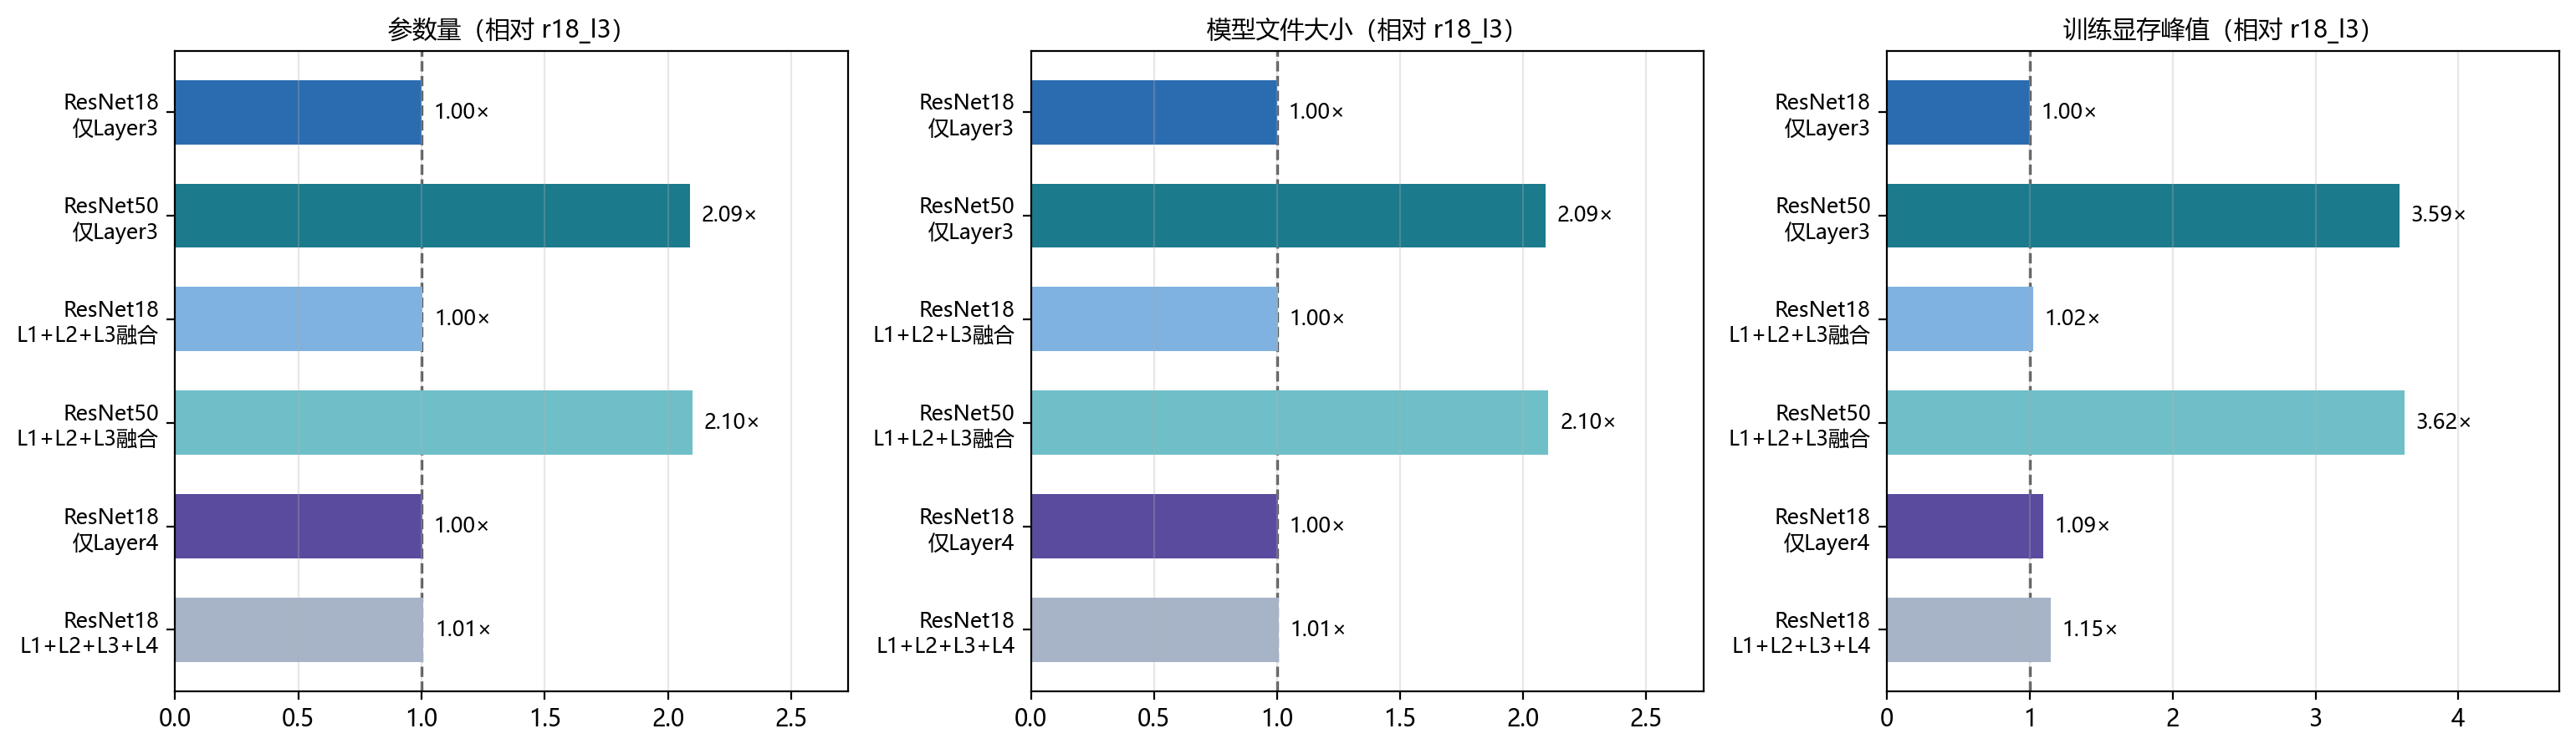
\includegraphics[width=0.88\textwidth]{fig4_cost_bar.png}
\caption{6 组配置的计算成本对比（参数量与模型大小为确定性量；\textbf{显存与 CPU 耗时为当前软硬件环境下重复测得}，随机器配置变化）}
\label{fig:cost}
\end{figure}

\noindent ResNet-50 相对 ResNet-18 的成本是\textbf{可精确测度的}：参数量 2.09 倍（11.37M $\rightarrow$ 23.75M）、模型文件 2.09 倍（43.5 $\rightarrow$ 90.9\,MB）、训练显存峰值 3.59 倍（622 $\rightarrow$ 2\,232\,MB）、\textbf{CPU 推理约 2.5 倍}（三组重复实测：r18\_l3 为 30.36/30.77/30.95\,ms，r50\_l3 为 77.72/78.15/79.51\,ms；\textbf{中位数之比 78.46/30.69 = 2.56}）。

\noindent 而它带来的精度收益是\textbf{不显著的}（IoU $p=0.2165$）。\textbf{用确定的两倍成本，去换一个测不出的收益，这不划算。}

\noindent\textbf{结论：}确定 \textbf{ResNet-18 + Layer3} 为当前方案。\textbf{这一选择是成本—精度权衡的结果}（在精度无可测差异的前提下，选参数量仅为一半、CPU 约 2.5 倍更快的那个），而非"更大的网络一定更好或一定更差"的普适判断。Lawley 等\cite{lawley2024network}在\textbf{腹部超声 16 类分类}任务上观察到"数据规模比网络选择更关键"，与本研究\textbf{方向一致}；\textbf{但该文任务、数据与指标均与本研究不同，不构成对本任务的直接验证，也不能据此断言"我们在本任务上无需再调网络"}。

\subsection{讨论一：为什么是 Layer3，而不是 Layer4}

\noindent\textbf{一、感受野实测（ResNet-18，输入 $384\times384$）。}按 $r_l = r_{l-1} + (k_l-1)\,J_{l-1}$ 逐层递推，且\textbf{只统计主干支路}（残差支路的 $1\times1$ 降采样卷积不扩大感受野，误计入会使感受野虚高约 4 倍）：Layer1--4 依次为 \textbf{43 / 99 / 211 / 435\,px}。\textbf{只有 Layer4（435\,px）首次超过输入高度 384\,px，Layer3 仅覆盖约 55\%}。

\noindent\textbf{二、加深并没有换来精度。}我们最初推导认为 Layer4 特征图仅 $12\times12$、量化误差下界 $s/2=16$\,px 必然超标，\textbf{但对照实验否定了它}：\texttt{r18\_l4} 上边界中位误差实测 \textbf{12.0\,px}，与 \texttt{r18\_l3} 的 11.2\,px 无显著差异（$p=0.8678$）。

\noindent\textbf{三、结论。}既然"覆盖全图"的 Layer4 与"只覆盖 55\%"的 Layer3 精度无可测差异，说明\textbf{对本任务而言感受野是否覆盖全图并非精度决定因素}——输入已在第一阶段裁成纯成像区，解剖上下文在局部与全局尺度上高度自相似。选 Layer3 是\textbf{成本—精度权衡}（$24\times24$ 而非 $12\times12$，纵向分辨率更细、算力更低），\textbf{而非"Layer4 不可能"或"Layer3 已全局"}。

\begin{figure}[htbp]
\centering
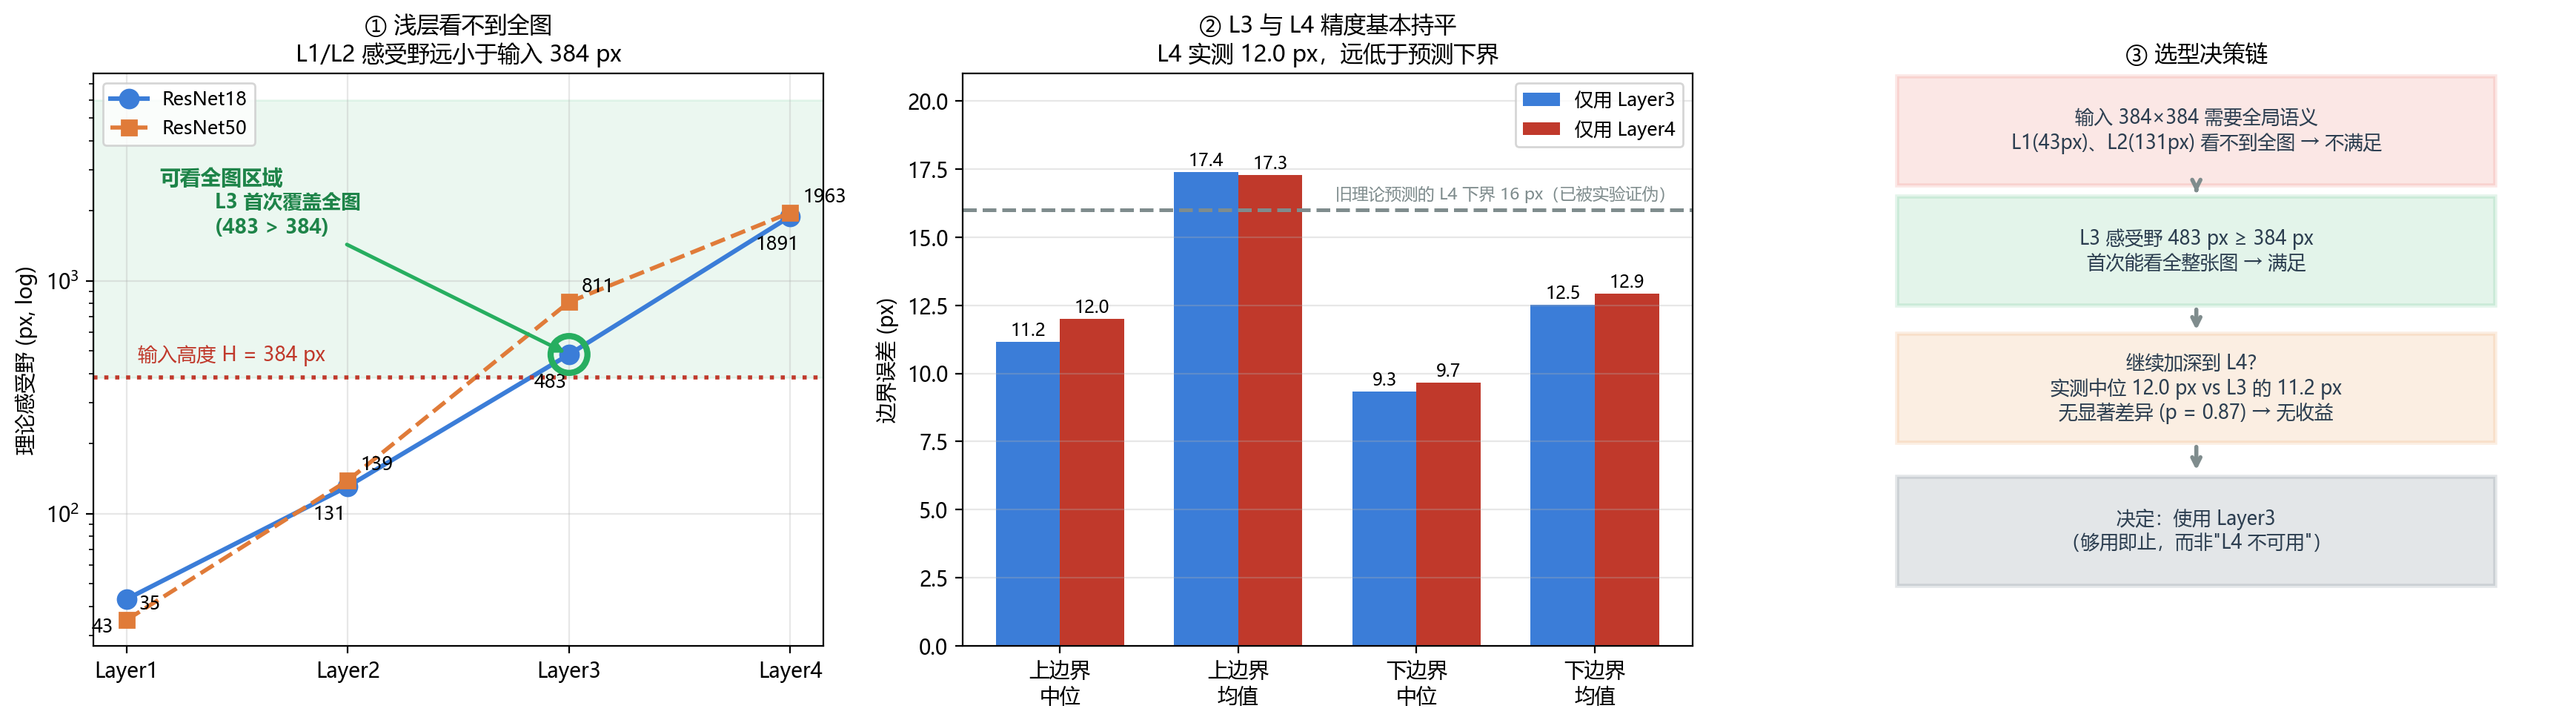
\includegraphics[width=0.7\textwidth]{fig_layer_selection_theory.png}
\caption{层级选择论证：左为感受野随深度增长（Layer1--4 依次为 43/99/211/435\,px，仅 Layer4 超过输入高度 384\,px）；中为 Layer3 与 Layer4 的实测精度对比，L4 远低于旧理论预测的下界；右为决策链}
\label{fig:layer}
\end{figure}

\subsection{讨论二：真正的突破在数据，不在模型}

这是本次实验最有价值的发现。

\begin{figure}[htbp]
\centering
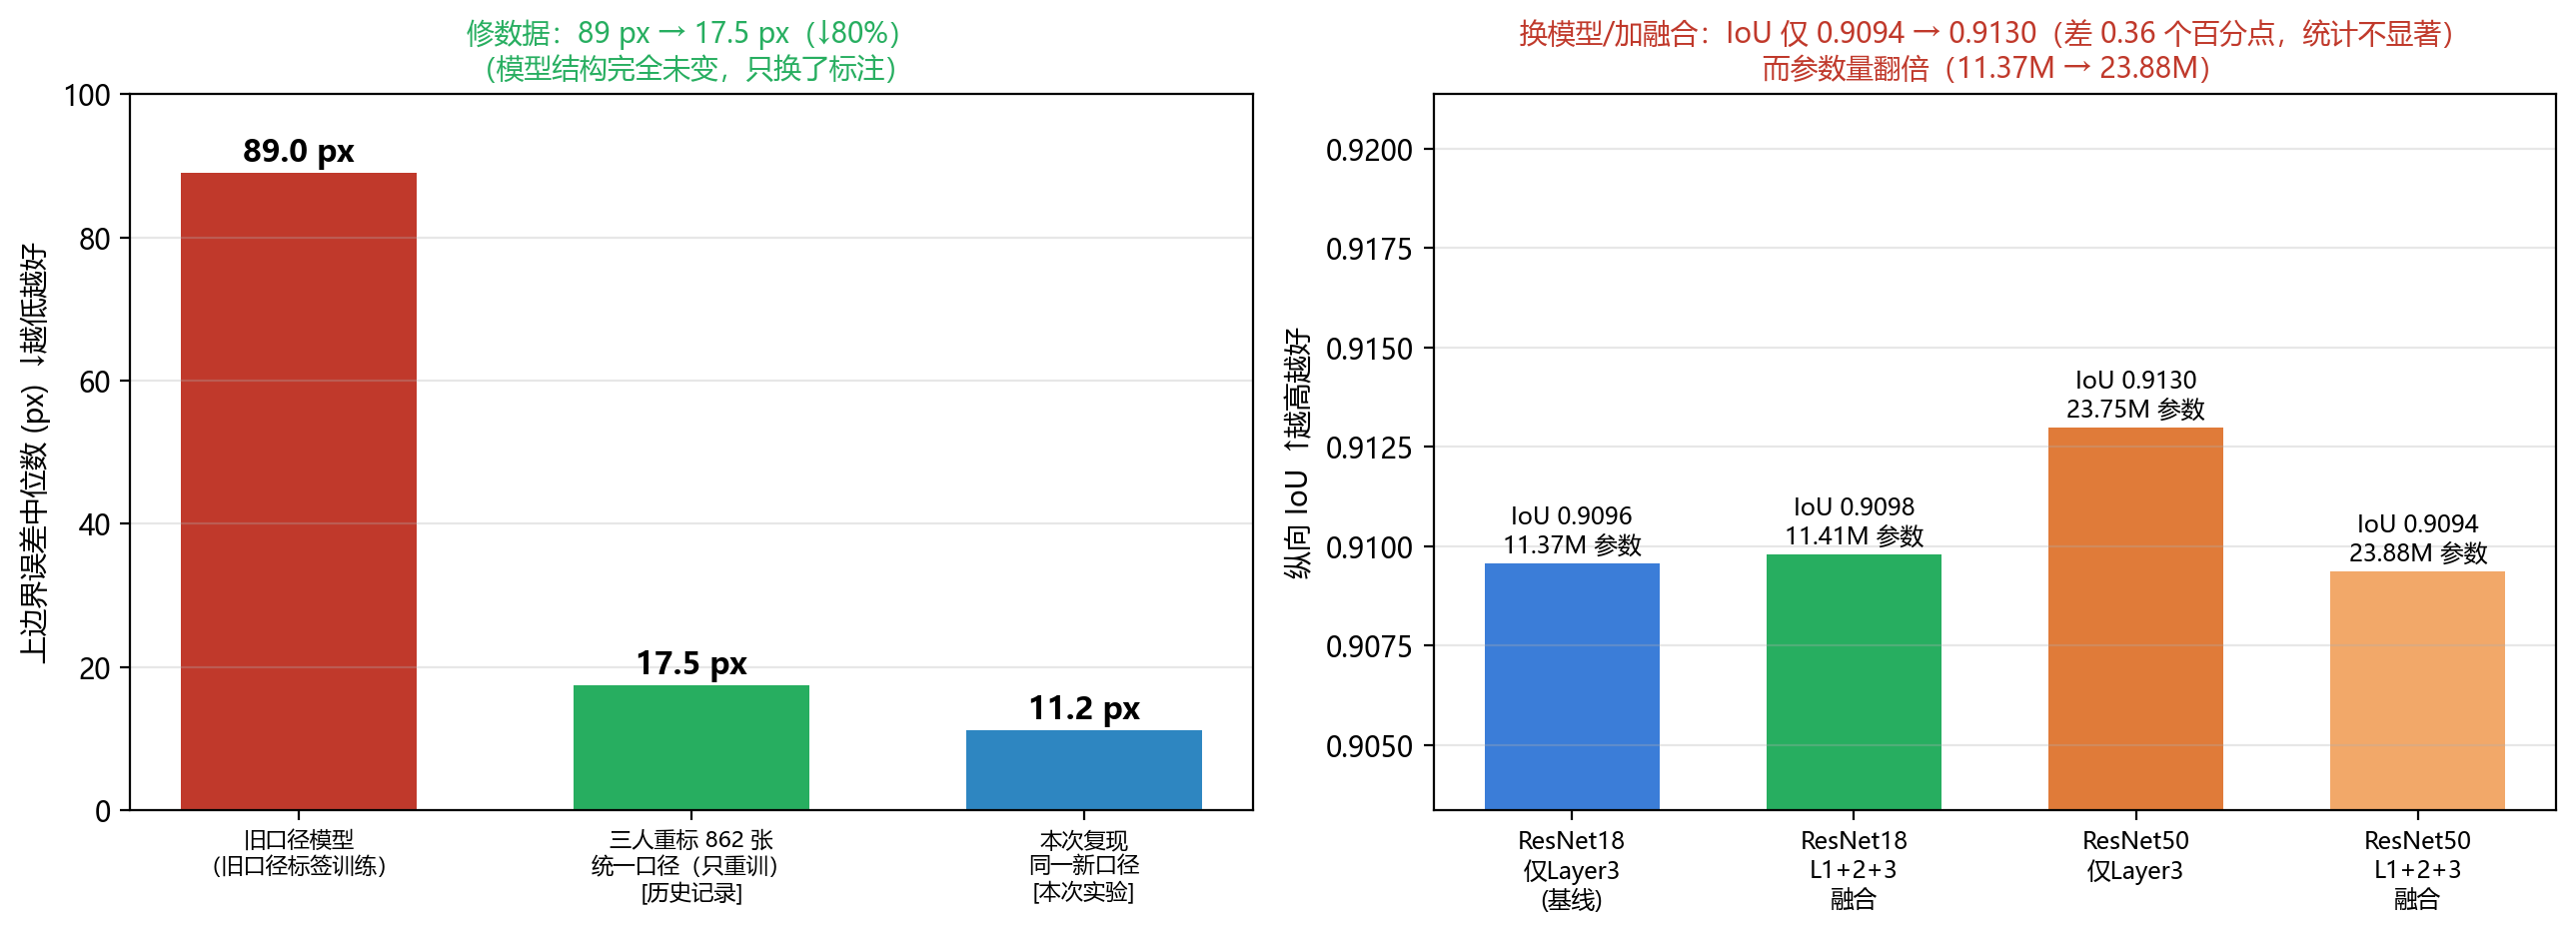
\includegraphics[width=0.72\textwidth]{fig_data_vs_model.png}
\caption{提升精度的两条路：修数据（左）远比换大模型（右）划算}
\label{fig:data}
\end{figure}

\begin{center}\small
\begin{tabular}{lccc}
\toprule
路径 & 精度变化 & 是否显著 & 代价 \\
\midrule
\textbf{统一标注口径} & 上边界\textbf{中位数} 89\,px $\rightarrow$ 17.5\,px（\textbf{↓80\%}） & -- & 人力标注 \\
换 ResNet-50 & IoU $+0.0034$ & 否（$p=0.22$） & 参数 2.09$\times$、推理 2.4$\times$ \\
加多尺度融合 & 3\% 合格率 $+5.7$\,pp & 否（$p=0.33$） & 参数 $+0.36\%$ \\
改用 Layer4 & 无变化 & 否（$p=0.87$） & -- \\
\bottomrule
\end{tabular}
\captionof{table}{提升精度的两条路线对比}
\end{center}

\noindent 模型结构完全未变、只把标注口径统一之后，上边界误差\textbf{中位数}从 89\,px 降到 17.5\,px，\textbf{降幅 80\%}——这是项目历史对照（旧口径 vs 新口径模型，同一测试集 88 张）。本次复现的新口径模型（表\ref{tab:summary}）上边界误差\textbf{均值 17.39\,px、中位数 11.2\,px}。\textbf{这两组数字不构成"口径已被验证正确"的证据}：历史记录 17.5\,px 是中位数，本次为 11.2\,px（低约 36\%），二者统计量与训练细节的一致性无法从现有记录完全确认。\textbf{唯一确定的是量级关系：口径修正带来的改善（89 $\rightarrow$ 17.5，约 5 倍）远大于任何结构改动（均在 1 个百分点或几个像素内）}。这与"图像质量与标准化对测量一致性的影响往往大于模型选择"这一普遍认识\cite{yu2021qualitycontrol}相符。\textbf{实践含义：把时间投入提高标注质量，比投入换更大模型，回报高得多。}





\subsection{不足与改进方向}

\noindent 我们如实列出四点局限：

\begin{enumerate}[leftmargin=1.6em,itemsep=2pt,topsep=2pt]
\item \textbf{人工标注标准难以机械性统一}。不同标注者对"成像区上边界该切在哪里"的判断存在细微差异，同一人在不同时间也会漂移；这类分歧靠算法消除不掉，需更明确的规范与多人交叉校验来收敛。目前\textbf{尚未计算标注者间一致性指标}（如 ICC），这是该局限的直接量化缺口。
\item \textbf{图像数量仍然有限}。本节对照实验使用的 862 张（训练集 560 张），是本轮所有"不显著"结论的直接背景；要验证多层级融合这类小幅改进，需要把数据量提上去。
\item \textbf{特殊 DDH 图像尚未充分适配}。部分截图的成像区内含无关文字与婴儿体位示意图，会被误当作成像内容，影响窗口定位与边界判断。系统目前用拒识标记把它们标为可疑，但\textbf{还没有做到良好的算法适配}，这是后续重点。
\item \textbf{尚未验证裁剪对测角精度的影响}。本文的 2\%/3\%/5\% 是\textbf{按窗口高度定义的工程阈值}，不是临床强制标准；项目\textbf{也尚未测量裁剪前后 Graf $\alpha$/$\beta$ 角的实际差异}。因此本文的结论止于"裁剪质量"，\textbf{不能外推为"已证明可提升临床测角一致性"}——这一环节需与临床合作方共同验证。
\end{enumerate}

\noindent\textbf{进一步的工作}：把特殊版式纳入窗口定位设计，并扩大数据规模、完善标注规范，让小幅改进也能被统计检验出来。


% ==================== 6 创新性说明 ====================
\section{创新性说明}

\subsection{问题定位：补上被忽视的前置环节}

现有 DDH 人工智能研究集中在\textbf{分型、测角、标准切面识别}等下游任务\cite{bhavsar2025ddh}，而\textbf{进入这些任务之前必需的图像裁剪环节长期被忽略}。本项目明确聚焦这一空白环节，将其定位为"为 Graf 分型及后续研究做前置准备"。这一定位的价值在于：\textbf{上游图像不规范，下游再好的模型也会被拖累}。

\subsection{方法设计：按误差性质拆分，让规则与学习各司其职}

我们没有采用"一个网络端到端搞定"的常见做法，而是按\textbf{误差性质}拆分任务：

\begin{itemize}[leftmargin=1.6em,itemsep=1.5pt,topsep=2pt]
\item \textbf{左右边界}是确定性几何量 $\rightarrow$ 交给规则算法，\textbf{无需训练、零样本可用、行为可解释}；
\item \textbf{上下边界}是模糊语义量 $\rightarrow$ 交给神经网络回归。
\end{itemize}

\noindent 这一设计的实际收益是：第一阶段不需要任何标注数据即可工作，\textbf{显著降低了冷启动成本}；同时规则部分失败模式可枚举，便于临床审计。而在网络内部，我们又做了两处"把约束写进结构"的设计：

\begin{itemize}[leftmargin=1.6em,itemsep=1.5pt,topsep=2pt]
\item \textbf{有序性由结构保证}：用\textbf{累积 softmax} 把上下边界表示为三段概率的累积和，使 $y_{\text{top}} \leq y_{\text{bot}}$ 恒成立，\textbf{从结构上消除了非法输出}，无需后处理修正；
\item \textbf{临床优先级写进目标函数}：非对称损失以 $w_{\text{in}}/w_{\text{out}} = 8$ 的比例惩罚\textbf{向内过裁}与\textbf{向外欠裁}，\textbf{把"宁可多留一点黑边，也不能切掉成像区"这一临床直觉，从口头约定变成了可优化的数学目标}。
\end{itemize}

\subsection{实验结论：用对照实验指出真正的突破口}

本次工作最有价值的产出，可能不是某个具体模型，而是一组\textbf{同等条件下的否定性结果}：在 560 张训练图的规模下，\textbf{换主干、加深层、多层级融合都没有产生统计显著的收益，而标注口径的统一带来误差显著下降}。该结论有 6 组同条件对照实验支撑，与文献\cite{lawley2024network}"数据规模比网络选择更关键"的观察\textbf{方向一致}（任务不同，不构成直接验证）。\textbf{结论边界须同时说明}：单一随机种子、88 张测试集、无多种子重复与预注册——它是"当前样本下未检出显著差异"，而非"已证明这些改动无效"。

\vspace{0.4em}


% ==================== 参考文献 ====================
\phantomsection
\begingroup
\footnotesize
\linespread{0.92}\selectfont
\setlength{\bibsep}{1pt plus 0.3pt}
\setlength{\parskip}{0pt}
\bibliographystyle{gbt7714-numerical}
\bibliography{refs_short}
\endgroup

\end{document}
